%===============================================================================
% LaTeX sjabloon voor de bachelorproef toegepaste informatica aan HOGENT
% Meer info op https://github.com/HoGentTIN/bachproef-latex-sjabloon
%===============================================================================

\documentclass{bachproef-tin}

\usepackage{hogent-thesis-titlepage} % Titelpagina conform aan HOGENT huisstijl
\usepackage{svg}
\usepackage{tcolorbox}
\usepackage{tikz}
\usetikzlibrary{positioning}
\usetikzlibrary{decorations.pathreplacing,calligraphy}
\usepackage{float}
\usepackage{booktabs}
\usepackage{xcolor}

%%---------- Documenteigenschappen ---------------------------------------------

% De titel van het rapport/bachelorproef
\title{Integratie van blockchain binnen een zelfontwikkeld ERP-systeem}

% Je eigen naam
\author{Arno Temmerman}

% De naam van je promotor (lector van de opleiding)
\promotor{Jan Willem}

% De naam van je co-promotor. Als je promotor ook je opdrachtgever is en je
% dus ook inhoudelijk begeleidt (en enkel dan!), mag je dit leeg laten.
\copromotor{Geert Borloo}

% Indien je bachelorproef in opdracht van/in samenwerking met een bedrijf of
% externe organisatie geschreven is, geef je hier de naam. Zoniet laat je dit
% zoals het is.
\instelling{14IT}

% Academiejaar
\academiejaar{2021-2022}

% Examenperiode
%  - 1e semester = 1e examenperiode => 1
%  - 2e semester = 2e examenperiode => 2
%  - tweede zit  = 3e examenperiode => 3
\examenperiode{2}

%===============================================================================
% Inhoud document
%===============================================================================

\begin{document}

%---------- Taalselectie -------------------------------------------------------
% Als je je bachelorproef in het Engels schrijft, haal dan onderstaande regel
% uit commentaar. Let op: de tekst op de voorkaft blijft in het Nederlands, en
% dat is ook de bedoeling!

%\selectlanguage{english}

%---------- Titelblad ----------------------------------------------------------
\inserttitlepage

%---------- Samenvatting, voorwoord --------------------------------------------
\usechapterimagefalse
%%=============================================================================
%% Voorwoord
%%=============================================================================

\chapter*{Woord vooraf}
\label{ch:voorwoord}

Deze bachelorproef werd uitgewerkt door Arno Temmerman met als doel het behalen van het diploma ``Professionele Bachelor: Toegepaste Informatica''. Een interesse in IT met een praktisch, maar wiskundig kantje brachten mij tot deze opleiding en uiteindelijk ook tot dit eindwerk.

Vooraleer ik tot de zaak kom, wil ik met dit voorwoord graag mijn opdrachte dank betuigen aan enkele mensen.

Eerst en vooral wil ik graag mijn promotor, Jan Willem, bedanken voor de begeleiding doorheen het hele onderzoeksproces. Zijn engagement en goede raad hebben me geholpen om deze scriptie tot een goed einde te brengen. De tweewekelijkse opvolgingsmomenten boden een zekere houvast en gaven me telkens een nieuwe insteek voor het vervolg van het onderzoek.

Daarnaast wil ik ook mijn copromotor, Geert Borloo, bedanken. Als mijn stagementor reikte hij me het onderwerp voor deze bachelorproef aan. Met zijn vakinhoudelijke kennis hielp hij me om het abstracte om te zetten in het concrete.

Tot slot wil ik graag nog het woord richten tot enkele mensen van het bedrijf mintBlue. Dankzij de vroegtijdige toegang tot hun platform kon ik een proof of concept uitwerken die nog tastbaarder was dan ik aanvankelijk durfde hopen. Bedankt Pieter Den Dooven, \mbox{Maurits} van Rijckevorstel en Niels van den Bergh om mijn interesse en vragen telkens met open armen te ontvangen.
%%=============================================================================
%% Samenvatting
%%=============================================================================

% TODO: De "abstract" of samenvatting is een kernachtige (~ 1 blz. voor een
% thesis) synthese van het document.
%
% Deze aspecten moeten zeker aan bod komen:
% - Context: waarom is dit werk belangrijk?
% - Nood: waarom moest dit onderzocht worden?
% - Taak: wat heb je precies gedaan?
% - Object: wat staat in dit document geschreven?
% - Resultaat: wat was het resultaat?
% - Conclusie: wat is/zijn de belangrijkste conclusie(s)?
% - Perspectief: blijven er nog vragen open die in de toekomst nog kunnen
%    onderzocht worden? Wat is een mogelijk vervolg voor jouw onderzoek?
%
% Max 1 bladzijde
%
% LET OP! Een samenvatting is GEEN voorwoord!

%%---------- Samenvatting -----------------------------------------------------
% De samenvatting in de hoofdtaal van het document

\chapter*{Samenvatting}

\lipsum[1-4]


%---------- Inhoudstafel -------------------------------------------------------
\pagestyle{empty} % Geen hoofding
\tableofcontents  % Voeg de inhoudstafel toe
\cleardoublepage  % Zorg dat volgende hoofstuk op een oneven pagina begint
\pagestyle{fancy} % Zet hoofding opnieuw aan

%---------- Lijst figuren, afkortingen, ... ------------------------------------

% Indien gewenst kan je hier een lijst van figuren/tabellen opgeven. Geef in
% dat geval je figuren/tabellen altijd een korte beschrijving:
%
%  \caption[korte beschrijving]{uitgebreide beschrijving}
%
% De korte beschrijving wordt gebruikt voor deze lijst, de uitgebreide staat bij
% de figuur of tabel zelf.

\listoffigures
\listoftables

% Als je een lijst van afkortingen of termen wil toevoegen, dan hoort die
% hier thuis. Gebruik bijvoorbeeld de ``glossaries'' package.
% https://www.overleaf.com/learn/latex/Glossaries

%---------- Kern ---------------------------------------------------------------

% De eerste hoofdstukken van een bachelorproef zijn meestal een inleiding op
% het onderwerp, literatuurstudie en verantwoording methodologie.
% Aarzel niet om een meer beschrijvende titel aan deze hoofstukken te geven of
% om bijvoorbeeld de inleiding en/of stand van zaken over meerdere hoofdstukken
% te verspreiden!

%%=============================================================================
%% Inleiding
%%=============================================================================

\chapter{Inleiding}
\label{ch:inleiding}

Sinds het grote succes van \textit{Bitcoin} is ``blockchain'' een vaste term geworden in het lexicon van de IT'er. Wat voor velen niet meer is dan een buzzwoord omtrent \textit{cyptogeld}, is voor anderen een trigger om te innoveren.
Die drang tot innovatie zet mensen ertoe aan om de technologie vanuit allerlei frisse invalshoeken te benaderen. Zodoende werd het toepassingsgebied van blockchain steeds uitgebreider, een proces dat nog volop aan de gang is. Ondernemers stellen zich de vraag of blockchain een meerwaarde kan bieden aan hun bedrijfsproces.

\section{Context}
\label{sec:context}

De insteek voor dit onderzoek kwam vanuit het softwarebedrijf 14IT. 14IT begon in 2014 met de ontwikkeling van CPSolution: een ERP-systeem door/voor kmo's. Een deel van het takenpakket bestaat uit het onderhouden en verder ontwikkelen van deze software. Binnen dit kader van \textit{continuous improvement} ontstond de interesse in dit onderwerp. Mede-eigenaar en copromotor Geert Borloo stelt zich de vraag of het programma verbeterd of uitgebreid kan worden door in te zetten op blockchaintechnologie. Vooral voor de dataopslag van facturen, contracten, abonnementen, ...  is 14IT benieuwd naar een mogelijke meerwaarde. Van hieruit ontstond de nood aan een onderzoek naar een mogelijke synergie tussen blockchain en ERP. 

\pagebreak

De doelstelling, zoals hierboven beschreven, kan herleid worden naar volgende onderzoeksvraag:

\begin{center}
	\textit{\textbf{``Hoe kunnen softwareontwikkelaars overgaan tot integratie van blockchaintechnologie voor de dataopslag van een ERP-systeem?''}}
\end{center}

In Hoofdstuk~\ref{ch:methodologie} -- \nameref{ch:methodologie} staat beschreven hoe deze onderzoeksvraag op een systematische manier werd beantwoord.



\section{Verantwoording}
\label{sec:verantwoording}

Opkomende technologieën vormen wel vaker de insteek van nieuwe projecten en onderzoeken. Een eerste doorbraak spreekt tot de verbeelding en zet aan tot innovatie. Op die manier kunnen echte hypes ontstaan, zoals bij blockchain het geval is. Dat maakt het nog belangrijker om het onderzoeksgebied van deze bachelorproef doelgericht af te bakenen. Uit analyses van Gartner blijkt namelijk dat het potentieel van hypetechnologieën gemakkelijk overschat wordt~\autocite{Kietzmann2018}. Een succesvol onderzoek slaagt erin om hype te onderscheiden van mogelijks rendabele toepassingen.

\begin{figure}[H]
	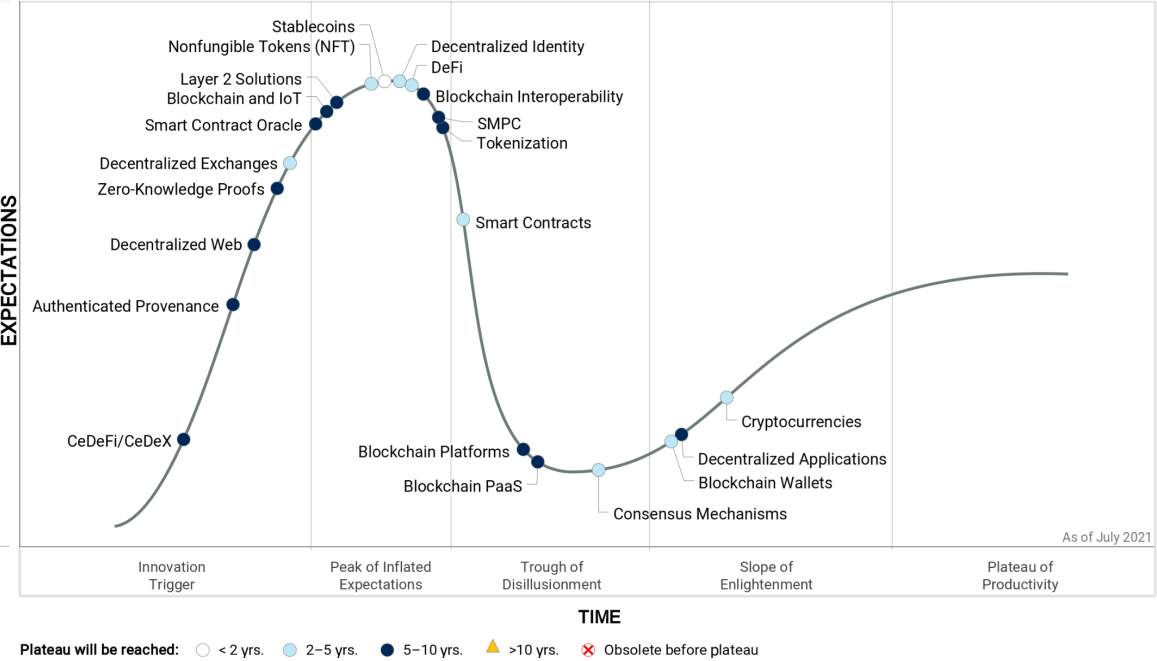
\includegraphics[width=\textwidth]{img/inleiding/gartner-hypecycle.png}
	\caption{\label{fig:gartner}Hype Cycle for Blockchain~\autocite{Gartner2021}}
\end{figure}

\pagebreak

In Figuur~\ref{fig:gartner} werd blockchain opgesplitst in 22 verschillende toepassingen. Elke toepassing werd voorgesteld als een punt op de Gartner Hype Cycle: een curve die weergeeft hoe de perceptie rond een hypetechnologie evolueert doorheen vijf vaste fases. Elk punt toont aan in welke fase de bijhorende toepassing zich bevindt (x-as) en als gevolg ook hoe hoog de verwachtingen errond zijn (y-as). De kleur van het punt stelt tevens een inschatting voor van hoe snel die toepassing matuur zal worden. 

Merk op dat 9 van de 22 toepassingen zich nog in de eerste opwaartse trend van de curve bevinden.
Die stijging wordt op gang getrokken door  een ``Innovation Trigger'' zoals een \textit{proof of concept} of belangstelling in de media. Men schat het potentieel heel hoog in, hoewel daar op dat moment nog weinig tot niets van in vervulling gebracht is. Hierdoor bereiken de verwachtingen al snel een maximum dat aanzienlijk hoger ligt dan wat de toepassing daadwerkelijk zal kunnen waarmaken: de ``Peak of Inflated Expectations''. Deze schromelijke overschatting zorgt gelukkig wel voor het nodige initiatief om de eerste commerciële projecten op poten te zetten. Een proces dat nog heel riskant is in dit ontwikkelingsstadium.

De ``Trough of Disillusionment'' maakt zijn intrede wanneer de eerste projecten niet het gewenste resultaat opleveren.
De verwachtingen van investeerders gaan de dieperik in door wat voor hen overkomt als mislukte experimenten. Desondanks is het een fase die zich aanbiedt als de geschikte gelegenheid tot onderzoek. Toepassingen, zoals ``Smart Contracts'' en ``Blockchain Platforms (aaS)'' komen stilaan \textit{down to earth} en vallen daarom mooi binnen de scope van deze paper. Een mix van succesverhalen en mislukkingen zorgen ervoor dat de grootste waanbeelden de deur uit zijn. De eerste commerciële implementaties doen hun intrede op de markt. Ze staan weliswaar nog in hun kinderschoenen, waardoor de vraag uit Sectie~\ref{sec:context} -- \nameref{sec:context} echt wel als een onderzoeksvraag mag beschouwd worden. 

In de huidige fase is het nog moeilijk om te beslissen of er mee op de trein gesprongen moet worden of niet. Met dit onderzoek kan hopelijk al een voorproefje gevonden worden van wat de ``Slope of Enlightenment'' zal brengen. Op die manier kan blockchain al benut worden voor de voordelen die binnen enkele jaren pas glashelder zullen worden. De ``Plateau of Productivity'' zal pas bereikt worden wanneer mainstream implementaties algemeen benut worden.

\newpage

\section{Opzet van deze bachelorproef}
\label{sec:opzet-van-deze-bachelorproef}

% Het is gebruikelijk aan het einde van de inleiding een overzicht te
% geven van de opbouw van de rest van de tekst. Deze sectie bevat al een aanzet
% die je kan aanvullen/aanpassen in functie van je eigen tekst.

De doelstelling van deze bachelorproef is om na te gaan of er een plaats is voor blockchain binnen het ERP-systeem van 14IT. Het is niet meteen duidelijk of het al dan niet haalbaar voor kmo's om data op te slaan in een blockchain. Daarnaast blijft ook nog de vraag of hier nuttige use cases voor weggelegd zijn. Om het onderzoek te laten slagen, was het van cruciaal belang om een resultaat na te streven dat praktisch bruikbaar is door 14IT. Dat gebeurde op twee manieren. 

Enerzijds moet dit werkstuk de lezer in staat stellen om zich op een vlotte manier in te werken in het onderwerp. Er valt al veel informatie te vinden over blockchains, waarvan niet even interessant is voor een ERP-systeem. De opbouw die in deze bachelorproef werd nagestreefd, zou 14IT moeten helpen om de state-of-the-art van het onderwerp snel te vatten.

Anderzijds biedt deze bachelorproef een \textit{proof of concept}. Deze zet de kennis en bevindingen van de sciptie om in een concrete toepassing. Het geeft 14IT een duidelijk beeld van wat mogelijk is binnen hun softwarepakket.


%%=============================================================================
%% Methodologie
%%=============================================================================

\chapter{Methodologie}
\label{ch:methodologie}

%% TODO: Hoe ben je te werk gegaan? Verdeel je onderzoek in grote fasen, en
%% licht in elke fase toe welke stappen je gevolgd hebt. Verantwoord waarom je
%% op deze manier te werk gegaan bent. Je moet kunnen aantonen dat je de best
%% mogelijke manier toegepast hebt om een antwoord te vinden op de
%% onderzoeksvraag.

Om de doelstelling van het onderzoek concreet te maken, werd volgende onderzoeksvraag geformuleerd:

\begin{center}
	\textit{\textbf{``Hoe kunnen softwareontwikkelaars overgaan tot integratie van blockchaintechnologie voor de dataopslag van hun ERP-systeem?''}}
\end{center}

Om op een systematische manier een antwoord te vinden op deze onderzoeksvraag, werd ze ontleed in vier deelvragen:

\begin{enumerate}
	\item Wat is een blockchain?
	\item Hoe wordt de data van het ERP-syteem opgeslagen? (\textit{as is})
	\item Welke mogelijkheden bieden blockchains voor een ERP-systeem?
	\item Hoe kunnen softwareontwikkelaars de data van hun ERP-systeem opslaan in een blockchain? (\textit{to be})
\end{enumerate}

Al van bij aanvang was het de bedoeling om, vertrekkende vanuit een high-level, zo snel mogelijk toe te werken naar de concrete bedrijfscasus. Die benadering weerspiegelt zich in de opgesomde deelvragen en de volgorde ervan.
Aan elk van de deelvragen werd een eigen hoofdstuk toegewijd.

Als eerste fase van het onderzoek, was het van cruciaal belang om een degelijk inzicht te verwerven in het onderwerp ``blockchain''. Dat gebeurde aan de hand van een \textbf{literatuurstudie} rond de eerste deelvraag van het onderzoek.
\textbf{Hoofdstuk~\ref{ch:blockchain} -- \nameref{ch:blockchain}} brengt de resultaten van deze studie samen, om de lezer zo de nodige achtergrond voor dit thema te bieden. Een rudimentaire implementatie van een blockchain wordt stap per stap opgebouwd, als oplossing voor een voorgedefiniëerde probleemstelling. Met deze opbouw komt de werking duidelijker naar voren. Dat is nodig om een gegrond inzicht te krijgen in de essentiële kenmerken van blockchains.

In \textbf{Hoofdstuk~\ref{ch:cpsolution} -- \nameref{ch:cpsolution}} werd het ERP-systeem van 14IT onder de loep genomen. Op die manier behandelt het de tweede deelvraag. Aan de hand van een \textbf{\textit{case study}} werd de huidige dataopslag van CPSolution in kaart gebracht. Daarmee werd het ``speelveld'' voor deze bachelorproef geconcretiseerd. Dat maakte het mogelijk om beter in te schatten welke noden, kansen en aandachtspunten er bestaan op vlak van dataopslag. Het was belangrijk om deze \textit{as-is} situatie voldoende te kennen, om zo gericht naar antwoorden op de volgende deelvraag te zoeken.

De voorgaande twee hoofdstukken leggen de basis voor de derde deelvraag. Deze wordt behandeld in \textbf{Hoofdstuk~\ref{ch:blockchaintoepassingen-voor-erp} -- \nameref{ch:blockchaintoepassingen-voor-erp}}. Aangezien zowel het begrip ``blockchain'' als ``ERP'' nu gekend is, kan gezocht worden naar een synergie tussen beide. Twee toepassingen uit de Gartner Hype Cycle\footnote{Zie Sectie~\ref{sec:verantwoording} -- \nameref{sec:verantwoording}.} geven de aanleiding tot NFT's, zo werd duidelijk uit een korte \textbf{literatuurverkenning}. Het kernidee dat tot de uiteindelijke \textit{proof of concept} leidde, is dat het mogelijk is om allerlei data in een blockchain op te nemen. Dat wordt geïllustreerd met een concreet voorbeeld van een NFT.

Een \textbf{\textit{proof of concept}} biedt het antwoord op de laatste deelvraag van het onderzoek. \textbf{Hoofdstuk~\ref{ch:proof-of-concept} -- \nameref{ch:proof-of-concept}} werd hieraan toegewijd. In dit hoofdstuk wordt een praktisch voorbeeld uitgewerkt van een blockchaintoepassing voor CPSolution. Hiervoor werd gesteund op de services van mintBlue, een bedrijf dat naar boven kwam bij een \textbf{marktverkenning} van het gekozen onderwerp.

Tenslotte, wordt in \textbf{Hoofdstuk~\ref{ch:conclusie} -- \nameref{ch:conclusie}} een antwoord geformuleerd op de overkoepelende onderzoeksvraag. 



% Voeg hier je eigen hoofdstukken toe die de ``corpus'' van je bachelorproef
% vormen. De structuur en titels hangen af van je eigen onderzoek. Je kan bv.
% elke fase in je onderzoek in een apart hoofdstuk bespreken.

\chapter{Blockchain}
\label{ch:blockchain}

% Tip: Begin elk hoofdstuk met een paragraaf inleiding die beschrijft hoe
% dit hoofdstuk past binnen het geheel van de bachelorproef. Geef in het
% bijzonder aan wat de link is met het vorige en volgende hoofdstuk.

Dit hoofdstuk is het resultaat van een literatuurstudie, toegespitst op de eerste deelvraag van het onderzoek:

\begin{center}
	\textit{\textbf{``Wat is een blockchain?''}}
\end{center}

Vertrekkende vanuit het \textit{double-spendingprobleem}, wordt geïllustreerd dat het delen van een grootboek \textit{of ledger} onvermijdelijk voor vertrouwenskwesties zorgt. Dit issue werd voor geruime tijd enkel vanuit een gecentraliseerd systeem benaderd. Met het verlangen naar de eerste \textit{cryptocurrencies} ontstond de nood aan een gedecentraliseerde benadering. Een blockchain vormde de oplossing voor de problemen die daarbij kwamen opdagen.

Volgende secties werden opgebouwd met als doel een inzicht te geven in de structuur van een blockchain en hoe zijn structuur tot stand kwam. Daarom wordt vertrokken vanuit een veralgemeende probleemstelling. Door deze \textit{case} stelselmatig aan te vullen met enkele basisprincipes komen we uiteinlijk tot een oplossing onder de vorm van een blockchain. Voor de uitwerking hiervan werd de implementatie van de eerste blockchain, zoals bedacht door Nakamoto, gebruikt als boegbeeld. Op die manier toont dit hoofdstuk hoe een blockchain aan zijn eigenschappen komt. Wie deze in het achterhoofd houdt, zal met een gefundeerd begrip de volgende deelvragen kunnen aanvatten.

% Pas na deze inleidende paragraaf komt de eerste sectiehoofding.


\section{Gedeelde ledgers}
\label{sec:gedeelde-ledgers}
In de whitepaper ``Bitcoin: A Peer-to-Peer Electronic Cash System'' werkte Satoshi Nakamoto het voorstel uit van wat men vandaag een blockchain noemt. Met een vernuftige keten van datablokken loste Nakamoto het zogenaamde \textit{double-spendingprobleem} op. Het \textit{incentive} was om Bitcoin, de eerste gedecentraliseerde cryptomunt, uit te brengen. Voor dit onderzoek is het echter zinvol om de context zo min mogelijk vast te hangen aan \textit{cryptocurrencies}. Daarom zullen we het begrip ``transacties'' ook opentrekken naar andere toepassingsgebieden. Een veralgemeende probleemstelling rond zogenaamde \textit{ledgers} zal het vertrekpunt vormen van een meer technische uiteenzetting.


\subsection{Double-spending}
\label{sub:double-spending}

Double-spending is een probleem binnen de context van \textit{cryptocurrencies}. Het doet zich voor wanneer een partij eenzelfde digitale token voor meerdere transacties gebruikt, hoewel dit maar voor een het geval zou mogen zijn~\autocite{Chohan2021}. Digitale munten kunnen namelijk (net zoals fysiek geld) gedupliceerd of vervalst worden. In tegenstelling tot tastbaar geld, bestaan digitale munten echter uitsluitend uit binaire data. Dat maakt de strijd tegen vervalsing extra uitdagend. Een kenteken van authenticiteit toevoegen, is op het eerste zicht niet mogelijk. Data kan namelijk heel gemakkelijk gerepliceerd worden. Een simpele aanduiding, analoog aan de zilverstrook op een bankbiljet, is bij een cryptomunt dus compleet zinloos. Het zou met een eenvoudige copy-paste kunnen vervalst worden~\autocite{Hoepman2008}. Om cryptomunten op de markt te brengen, waren dus andere oplossingen nodig.


\subsection{Transacties}
\label{sub:transacties}

Een transactie staat voor een interaction tussen partijen~\autocite{Salem2008}. In de oorspronkelijke toepassing van blockchains betekende dit de bitcoin-overdracht van een partij naar een andere~\autocite{Pierro2017}. Er zijn echter veel meer transacties denkbaar dan enkel eenvoudige gelduitwisselingen.
In het boek ``Blockchain: Blueprint for a New Economy'' wordt blockchain-technologie opgedeeld in drie fases. De bijhorende toepassingsgebieden bepalen de transacties die denkbaar zijn om op te nemen in een blockchain~\autocite{Swan2015}.

\textbf{Blockchain 1.0} is het label voor blockchain-technologie, zoals die bestond in zijn oorspronkelijke context: cryptocurrencies. Een transactie staat in die context voor
\begin{itemize}
	\item het spenderen van een cryptomunt.
\end{itemize}
\textbf{Blockchain 2.0} staat voor een uitbreiding van de technologie, die voornamelijk beperkt blijft tot de financiële sector. Banken, betalingen en de \textit{supply chain} geven aanleiding tot transacties zoals
\begin{itemize}
	\item afsluiten van \textit{smart contracts}
	\item uitwisselen van aandelen;
	\item uitwisselen van hypotheken;
	\item afsluiten van een abonnement;
	\item afsluiten van een verzekering;
	\item het versturen van een digitale factuur;
	\item ...
\end{itemize}
\textbf{Blockchain 3.0} wordt beschreven als de toepassing van blockchain in sectoren zoals gezondheidszorg, wetenschap, cultuur en de overheid~\autocite{Xu2019}. De uitwisseling die dan plaatsvindt gaat niet zozeer over financiële zaken, maar over informatie die ontstaat bij
\begin{itemize}
	\item de waarnemingen van een metaaldetector bij voedingsproductie;
	\item het toedienen van een inenting;
	\item het indienen van een subsidieaanvraag bij de overheid;
	\item ...
\end{itemize}

Ook al deze zaken horen uiteraard onvervalsbaar te zijn. Door het begrip transactie ruimer te bekijken, kan double-spending vertaald worden naar veralgemeende probleemstelling. Dit is zinvol, aangezien de \textit{use cases} voor dit onderzoek niet te vinden zijn in Blockchain 1.0, maar starten bij Blockchain 2.0.


\subsection{Probleemstelling}
\label{sub:probleemstelling}

In de gegeven context kunnen drie partijen onderlinge transacties uitvoeren. Er ontstaat nood aan een gedeeld grootboek of \textit{ledger} om al deze transacties in op te nemen. In deze ledger moet elke partij
\begin{itemize}
	\item nieuw uitgevoerde transacties kunnen opslaan;
	\item de voorgaande transacties kunnen raadplegen.
\end{itemize}

De ledger moet uiteraard betrouwbaar zijn. Dit wil zeggen dat er geen vervalste of gedupliceerde regels mogen voorkomen in de ledger.

\begin{figure}[H]
	\centering
	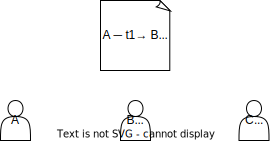
\includegraphics[]{img/blockchain/probleemstelling.pdf}
	\caption{\label{fig:probleemstelling}Probleemstelling}
\end{figure}

\begin{tcolorbox}[title=Voorbeeld]	
Partij A voert een transactie uit met partij B. Partij A schrijft de transactie weg in de ledger.

Partij C voert een transactie uit met partij A. Partij C schrijft de transactie weg in de ledger.
\end{tcolorbox}

Er schuilt een inherente vertrouwenskwestie in het bijhouden van een gedeelde ledger: alle deelnemedende partijen moeten elkaar vertrouwen. Volgende kwestie lijkt op het double-spendingprobleem bij cryptomunten:

\textbf{Probleem:} 
Partij A voert geen transactie uit met partij B, maar schrijft toch een lijn weg in de ledger. Partij B gaat hier uiteraard niet mee akkoord. Voor partij C lijkt het alsof er nog een transactie plaatsvond tussen A en B.


\subsection{Centralized ledger}
\label{sub:centralized-ledger}

Voorgaande probleemstelling werd traditioneel aangepakt vanuit een gecentraliseerd systeem. Er wordt een onafhankelijke partij ingeschakeld voor het bijhouden en bewaken van de ledger~\autocite{Rawat2020}. Deze derde partij houdt de ledger bij op een centrale databank die raadpleegbaar is door alle andere partijen. Wie een transactie wilt wegschrijven in de ledger, doet een aanvraag die kan gecheckt worden. Op die manier waakt de centrale partij erover dat er enkel geldige en geverifieerde transacties in de ledger kunnen komen. 

Om te authenticiteit van een transactie aan te tonen wordt in de praktijk gebruik gemaakt van een \textit{digital signature}~\autocite{Salem2008}. Het vormt de oplossing voor het \textit{copy-pasteprobleem} dat werd aangehaald in subsectie \ref{sub:double-spending} - \nameref{sub:double-spending}. Door bij elke regel een unieke code te gegenereren op basis van een publieke en private sleutel, kan deze later geverifiëerd worden\footnote{Een diepgaandere uiteenzetting van \textit{digital signatures} is in dit onderzoek niet aan de orde.}. Net zoals een handtekening bij fysieke documenten, wordt zo de probleemstelling aangepakt.

\begin{figure}[H]
	\centering
	\includegraphics[]{img/blockchain/centralized-ledger.pdf}
	\caption{\label{fig:centralized-ledger}Centralized ledger}
\end{figure}

Merk op dat de probleemstelling in principe niet volledig opgelost is. De vertrouwenskwestie die partijen onderling hadden, is in zekere zin gewoon verschoven naar het nieuwe, centrale figuur. Dit kan gezien worden als een Single Point of Failure~\autocite{Majaski2021}.

\textbf{Probleem:} 
Op vraag van partij A verwijdert het centrale figuur een voorgaande transactie tussen A en B. 
Aangezien dit de enige kopie is van de ledger is er geen manier voor partij B om hierop terug te komen. Parij C weet niets over het hele scenario.

Met een gedistribueerd systeem kan men de nood aan een centrale authoriteit proberen vermijden.


\subsection{Distributed ledger}
\label{sub:distributed-ledger}

Om de nood aan een centrale opslagplaatst te omzeilen, zou elke partij een eigen kopie kunnen bijhouden van de gezamenlijke ledger. Zo kan elke partij over zijn kopie waken en valse transacties onderscheppen. Om een nieuwe regel toe te voegen aan de ledger, wordt een signaal \textit{gebroadcast} op het netwerk. De ontvangende partijen kunnen hierna hun versie van de ledger updaten~\autocite{Nakamoto2008}. Hierdoor ontstaat echter een nieuw probleem.

\begin{figure}[H]
	\centering
	\includegraphics[]{img/blockchain/distributed-ledger.pdf}
	\caption{\label{fig:distributed-ledger}Distributed ledger}
\end{figure}

\textbf{Probleem:} Partij A voert een transactie uit met partij B, maar broadcast dit niet naar partij C. De ledger van partij C stemt niet meer overeen met die van A en B.

Hoewel het handig is dat elke partij zijn eigen versie van de gedeelde ledger heeft, laat dit een nieuwe vraag ontstaan: wat is ``de juiste'' versie? Om transacties correct bij te houden in een gedistribueerd systeem, is er nood aan een protocol, een technologie die deelnemende partijen een manier biedt om het eens te zijn over wat de correcte ledger is. Die technologie staat bekend als een blockchain~\autocite{Chaudhry2018}.


\section{Uitgangspunten}
\label{sec:uitgangspunten}

De blockchain kwam als oplossing voor het probleem dat beschreven wordt in subsectie \ref{sub:distributed-ledger} - \nameref{sub:distributed-ledger}. Zoals reeds aangegeven, werd dit probleem voor het eerst opgelost bij de ontwikkeling van de Bitcoin. Om een gegrond inzicht te geven in de eigenschappen van een blockchain, is deze sectie opgedeeld in drie basisprincipes. De concrete invulling van die principes is gebaseerd op de oorspronkelijke implementatie door Nakamoto.

Volgende subsecties zullen aantonen hoe het vertrouwensprobleem bij een \textit{distributed ledger} kan opgelost worden door het gezamenlijk opstellen van een keten van datablokken: een proces genaamd mining.


\subsection{Blokken}
\label{sub:blokken}

Een eerste basisprincipe is dat de ledger wordt opgebouwd uit zogenaamde blokken die elk een apart deel van de transacties oplijsten. Deze blokken worden om de zoveel tijd gegenereerd door een proces dat ``mining'' genoemd wordt~\autocite{Bhaskar2015}.

Tijdens het minen, wordt gedurende een beperkte tijdsspanne geluisterd naar de transacties die gebroadcast worden over het netwerk. Het blok houdt deze transacties dan bij onder de vorm van een Merkle Tree\footnote{Deze speciale binaire boom maakt handig gebruik van hashing om de transacties van het blok snel valideerbaar te maken. Deze datastructuur wordt uitsluitend gebruikt binnen een blok. Om verwarring te vermijden met de structuur van de blockchain als geheel, wordt deze verder niet besproken.}~\autocite{Salem2008}. Op die manier omvat het een uniek deel van de ledger. Wanneer de tijdslimiet verstreken is, kan de opbouw van het blok afgerond worden~\autocite{Nakamoto2008}. Hierbij gebeuren nog een aantal essentiële stappen die in de volgende subsecties besproken worden. 

Wanneer een blok klaar is, wordt het in zijn geheel \textit{gebroadcast}, waarna het door de deelnemers van het netwerk kan geaccepteerd worden~\autocite{Nakamoto2008}. Zo wordt de distributed ledger stuk per stuk aangevuld.
Om deze stukken aan elkaar te linken, zal elk blok ook een verwijzing krijgen naar zijn voorganger. Voor deze verwijzing wordt gebruik gemaakt van een cryptografische hashfunctie. 

\begin{figure}[H]
	\centering
	\includegraphics[]{img/blockchain/blokken.pdf}
	\caption{\label{fig:blokken}Gedeelde ledger, opgedeeld in blokken}
\end{figure}

\subsection{Cryptohashes}
\label{sub:cryptohashes}

Naast een lijst van transacties, houdt elk blok ook een verwijzing bij naar het voorgaande blok. Deze verwijzing is onder de vorm van een hashwaarde die bepaald wordt door een hashfunctie zoals SHA-256~\autocite{Nakamoto2008}. Wanneer die functie een blok als input krijgt, geeft deze een binaire tekenreeks van vaste lengte als output~\autocite{Slaats2019}. Die tekenreeks wordt dan gebruikt als verwijzing naar het voorgaande blok. Op die manier komt men tot een keten van blokken: een blockchain.

\begin{center}
	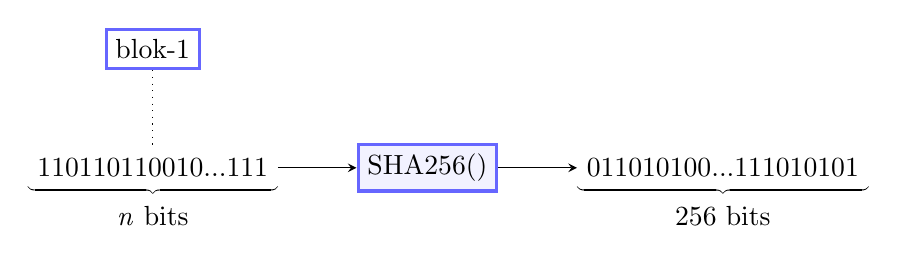
\begin{tikzpicture}[
		roundnode/.style={circle, draw=green!60, fill=green!5, very thick, minimum size=7mm},
		squarednode/.style={rectangle, draw=blue!60, fill=blue!5, very thick, minimum size=5mm},
		]
		%Nodes
		\node[squarednode,fill=none]  (blok-1)        					    {blok-1};
		\node[draw=none,fill=none]    (input)         [below=of blok-1]       {110110110010...111};
		\node[draw=none,fill=none]    (output-length) [below=of input, yshift=25]		{\textit{n} bits};
		\node[squarednode]            (sha256) 		  [right=of input]       {SHA256()};
		\node[draw=none,fill=none]    (output)        [right=of sha256]		{011010100...111010101};
		\node[draw=none,fill=none]    (output-length) [below=of output, yshift=25]		{256 bits};
		
		% Calligraphic brace
		\draw [decorate, decoration = {calligraphic brace}] (input.south east) --  (input.south west);
		\draw [decorate, decoration = {calligraphic brace}] (output.south east) --  (output.south west);
		
		%Lines
		\draw[dotted] (blok-1.south) -- (input.north);
		\draw[-stealth] (input.east) -- (sha256.west);
		\draw[-stealth] (sha256.east) -- (output.west);
		
	\end{tikzpicture}
\end{center}

Voor elke input van de hashfunctie, kan eenvoudig de output bepaald worden. Toch is het geheel onwezenlijk om de inverse berekening te maken. Daarom wordt deze hashfunctie cryptografisch genoemd. Dit is een van de sleutelkenmerken die blockchain mogelijk maken: het is niet haalbaar om de input van een gegeven hashwaarde te \textit{reverse-engineeren}~\autocite{Mansfield2018}. 

Het is belangrijk om erop te wijzen dat zelfs de kleinste wijziging aan de input van een hashfunctie, een drastisch verschil maakt aan de output. In deze context betekent dit dat een wijziging aan een blok (hoe klein dan ook) ervoor zorgt dat zijn hashwaarde volledig verandert. Aangezien deze hashwaarden gebruikt worden om de blokken aan elkaar te ketenen, zal de blockchain hierdoor ergens doorbroken worden. De hashwaarde die naar dit blok verwees is namelijk niet meer correct.~\autocite{Salem2008} Om terug tot een geldige blockchain te komen zal er een hele kettingreactie moeten plaatsvinden. Onderstaand voorbeeld illustreert waarom dit het geval is:

\begin{tcolorbox}[title=Voorbeeld]	
	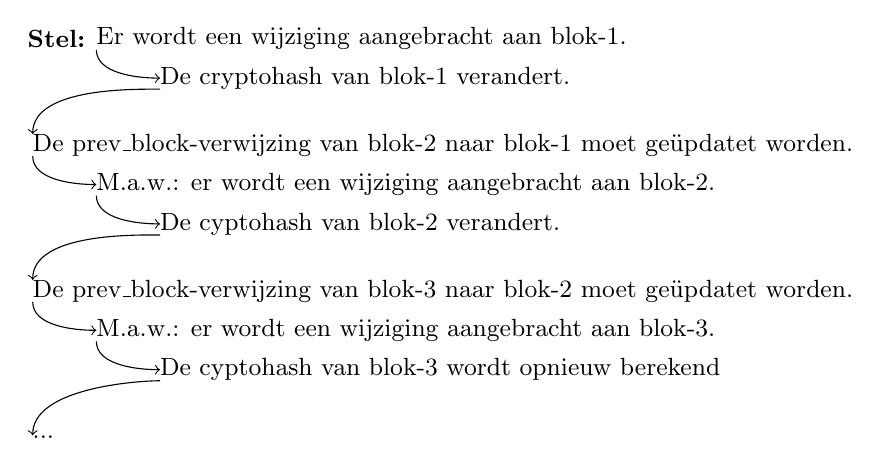
\begin{tikzpicture}[every node/.style={inner sep=0,outer sep=0, font=\small}, align=left, node distance=.5]
		
		%Nodes
		\node[draw=none,fill=none] (11)        					    {\textbf{Stel: }};
		\node[draw=none,fill=none] (12) [right=of 11, xshift=-15] {Er wordt een wijziging aangebracht aan blok-1.};
		\node[draw=none,fill=none] (13) [below=of 12.west, anchor=west, xshift=23] {De cryptohash van blok-1 verandert.};
		\node[draw=none,fill=none] (21) [below=of 13.west, anchor=west, xshift=-46, yshift=-10]  {De prev\_block-verwijzing van blok-2 naar blok-1 moet geüpdatet worden.};
		\node[draw=none,fill=none] (22) [below=of 21.west, anchor=west, xshift=23]  {M.a.w.: er wordt een wijziging aangebracht aan blok-2.};
		\node[draw=none,fill=none] (23) [below=of 22.west, anchor=west, xshift=23]  {De cyptohash van blok-2 verandert.};
		\node[draw=none,fill=none] (31) [below=of 23.west, anchor=west, xshift=-46, yshift=-10]  {De prev\_block-verwijzing van blok-3 naar blok-2 moet geüpdatet worden.};
		\node[draw=none,fill=none] (32) [below=of 31.west, anchor=west, xshift=23]  {M.a.w.: er wordt een wijziging aangebracht aan blok-3.};
		\node[draw=none,fill=none] (33) [below=of 32.west, anchor=west, xshift=23]  {De cyptohash van blok-3 wordt opnieuw berekend};
		\node[draw=none,fill=none] (41) [below=of 33.west, anchor=west, xshift=-46, yshift=-10]  {...};
		
		%Lines
		\draw[->] (12.south west) .. controls +(down:3mm) and +(left:3mm) .. (13.west);
		\draw[->] (13.south west) .. controls +(left:3mm) and +(up:6mm) .. (21.north west);
		\draw[->] (21.south west) .. controls +(down:3mm) and +(left:3mm) .. (22.west);
		\draw[->] (22.south west) .. controls +(down:3mm) and +(left:3mm) .. (23.west);
		\draw[->] (23.south west) .. controls +(left:3mm) and +(up:6mm) .. (31.north west);
		\draw[->] (31.south west) .. controls +(down:3mm) and +(left:3mm) .. (32.west);
		\draw[->] (32.south west) .. controls +(down:3mm) and +(left:3mm) .. (33.west);
		\draw[->] (33.south west) .. controls +(left:3mm) and +(up:6mm) .. (41.north west);
	\end{tikzpicture}	
\end{tcolorbox}

Bovenstaand voorbeeld toont aan dat de inhoud van een blok niet gewijzigd kan worden, zonder ook alle daaropvolgende blokken te wijzigen. Het gaat namelijk steeds gepaard met de wijziging van de bijhorende hash. Aangezien deze hash altijd deel uitmaakt van een daaropvolgend blok, zullen al deze verwijzingen moeten herberekend worden~\autocite{Nakamoto2008}.

Niemand zal nog een aanpassing kunnen maken aan de ledger zoals:
\begin{itemize}
	\item een transactie wijzigen, toegevoegen of verwijderen;
	\item het verwisselen van transacties;
	\item het verwisselen van blokken;
\end{itemize}

zonder verantwoordelijk te worden voor alle hashverwijzingen na het geïmpacteerde punt. Op die manier wordt al een eerste stap gezet naar een onvervalsbare, of \textit{immutable} \textit{distributed ledger}. Het doel is echter nog niet bereikt.

\textbf{Probleem:} 
Wie de ledger wenst te vervalsen hoeft zich geen zorgen te maken over het doorbreken van de keten. 
Door simpelweg de nodige hashes opnieuw te berekenen, komt men uiteindelijk terug tot een geldige blockchain. Dat kan, aangezien uitvoeren van een hashfunctie in constante tijd kan gebeuren~\autocite{Slaats2019}. Op die manier kunnen nog steeds tegenstrijdige, maar technisch geldige ledgers ontstaan.

Een laatste essentieel principe bestaat eruit om bij elk blok een extra speciaal stuk data te eisen, waardoor het vinden van een gepaste hash wel een rekenintesieve opdracht wordt. Op die manier wordt ook het bovenstaande probleem opgelost.

\begin{figure}[H]
	\centering
	\includegraphics[]{img/blockchain/blokken-met-cryptohash.pdf}
	\caption{\label{fig:blokken-met-cryptohash}Blokken met een cryptohash als verwijzing}
\end{figure}

\subsection{Proof of Work}
\label{sub:proof-of-work}

De laatste sleutel bestaat eruit om een extra stukje data toe te voegen aan elk blok genaamd de ``Proof of Work''.
Afhankelijk van de inhoud van die Proof of Work, zal het blok uiteraard veranderen, en als gevolg ook de hash van dat blok~\autocite{Nakamoto2008}. Met andere woorden: door dit stukje data te tweaken, wijzigt men de hash die nodig is om te verwijzen naar dat blok.

Het opzet is om nu een extra vereiste op te leggen aan die hashverwijzingen, zodat het tijdrovend wordt om die PoW te produceren. Nakamoto vond een dergelijke vereiste, die desondanks eenvoudig is om te verifiëren: de has moet beginnen met een voorgedefiniëerd aantal nul-bits. Een blok zal pas als geldig beschouwd worden, wanneer de eerste \textit{x} bits allemaal de waarde nul hebben. 

\begin{center}
	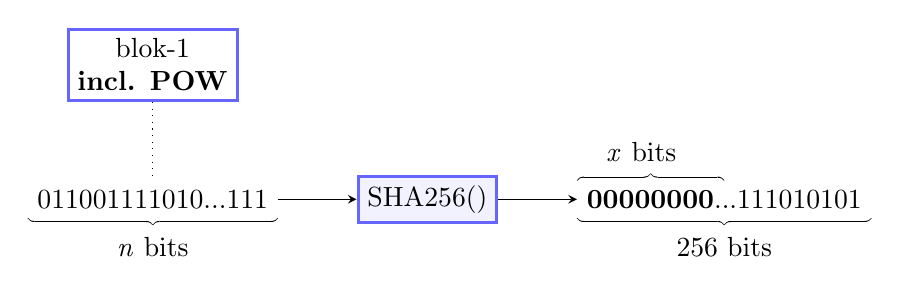
\begin{tikzpicture}[
		roundnode/.style={circle, draw=green!60, fill=green!5, very thick, minimum size=7mm},
		squarednode/.style={rectangle, draw=blue!60, fill=blue!5, very thick, minimum size=5mm},
		]
		%Nodes
		\node[squarednode,fill=none, align=center]  (blok-1)        					    {blok-1\\\textbf{incl. POW}};
		\node[draw=none,fill=none]    (input)         [below=of blok-1]       {011001111010...111};
		\node[draw=none,fill=none]    (output-length) [below=of input, yshift=25]		{\textit{n} bits};
		\node[squarednode]            (sha256) 		  [right=of input]       {SHA256()};
		\node[draw=none,fill=none]    (output)        [right=of sha256]		{\textbf{00000000}...111010101};
		\node[draw=none,fill=none]    (output-length) [above=of output, xshift=-30, yshift=-25]		{\textit{x} bits};
		\node[draw=none,fill=none]    (output-length) [below=of output, yshift=25]		{256 bits};
		
		% Calligraphic brace
		\draw [decorate, decoration = {calligraphic brace}] (input.south east) --  (input.south west);
		\draw [decorate, decoration = {calligraphic brace}] (output.north west) --  (output.north);
		\draw [decorate, decoration = {calligraphic brace}] (output.south east) --  (output.south west);
		
		%Lines
		\draw[dotted] (blok-1.south) -- (input.north);
		\draw[-stealth] (input.east) -- (sha256.west);
		\draw[-stealth] (sha256.east) -- (output.west);
	\end{tikzpicture}
\end{center}

Om tot een geldig blok te komen, zal dus telkens een PoW-waarde gezocht moeten worden, die de hash van dat blok laat starten met de nodige nulbits. Aangezien het hier over een cryptografische hasahfunctie gaat, valt die Proof of Work niet zomaar te voorspellen~\autocite{Mansfield2018}. Er zit niets anders op dan herhaaldelijk willekeurige waarden uit te proberen, tot er toevallig een geldige hashwaarde uit voortkomt.

\begin{flushright}
	\textit{{\small ``The proof-of-work involves scanning for a value that when hashed, such as with SHA-256, the hash begins with a number of zero bits. The average work required is exponential in the number of zero bits required and can be verified by executing a single hash.''}}
	
	~\autocite{Nakamoto2008}
\end{flushright}

Onderstaand voorbeeld illustreert hoe de kettingreactie bij het wijzigen van een blok er nu uitziet:

\begin{tcolorbox}[title=Voorbeeld]	
	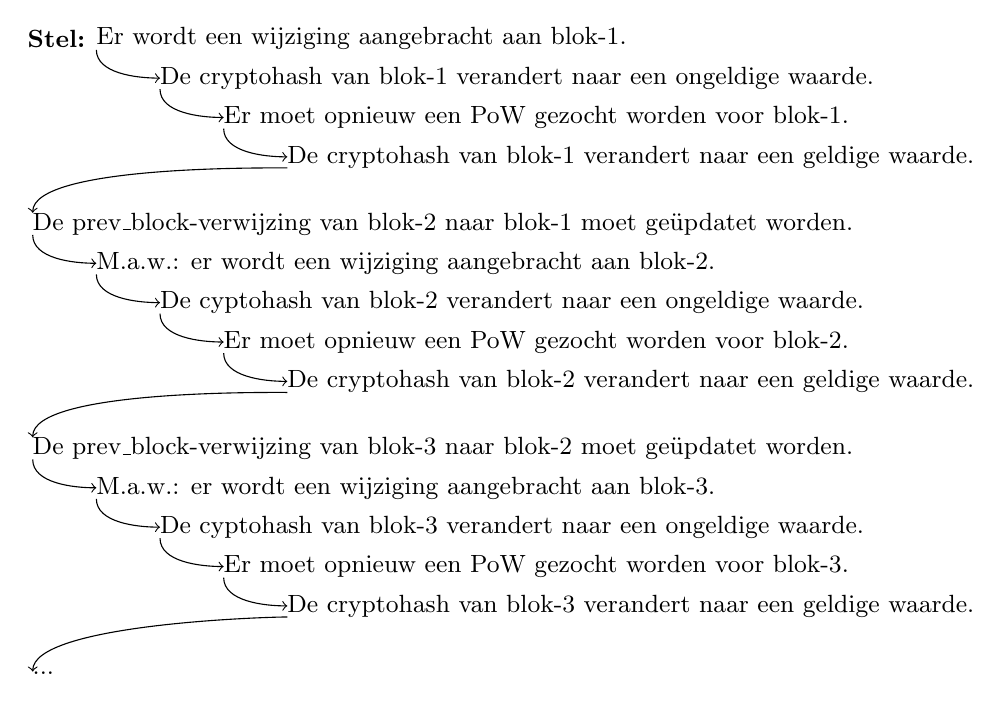
\begin{tikzpicture}[every node/.style={inner sep=0,outer sep=0, font=\small}, align=left, node distance=.5]
		
		%Nodes
		\node[draw=none,fill=none] (11)        					    {\textbf{Stel: }};
		\node[draw=none,fill=none] (12) [right=of 11, xshift=-15] {Er wordt een wijziging aangebracht aan blok-1.};
		\node[draw=none,fill=none] (13) [below=of 12.west, anchor=west, xshift=23] {De cryptohash van blok-1 verandert naar een ongeldige waarde.};
		\node[draw=none,fill=none] (14) [below=of 13.west, anchor=west, xshift=23] {Er moet opnieuw een PoW gezocht worden voor blok-1.};
		\node[draw=none,fill=none] (15) [below=of 14.west, anchor=west, xshift=23] {De cryptohash van blok-1 verandert naar een geldige waarde.};
		\node[draw=none,fill=none] (21) [below=of 15.west, anchor=west, xshift=-92, yshift=-10]  {De prev\_block-verwijzing van blok-2 naar blok-1 moet geüpdatet worden.};
		\node[draw=none,fill=none] (22) [below=of 21.west, anchor=west, xshift=23]  {M.a.w.: er wordt een wijziging aangebracht aan blok-2.};
		\node[draw=none,fill=none] (23) [below=of 22.west, anchor=west, xshift=23]  {De cyptohash van blok-2 verandert naar een ongeldige waarde.};
		\node[draw=none,fill=none] (24) [below=of 23.west, anchor=west, xshift=23] {Er moet opnieuw een PoW gezocht worden voor blok-2.};
		\node[draw=none,fill=none] (25) [below=of 24.west, anchor=west, xshift=23] {De cryptohash van blok-2 verandert naar een geldige waarde.};
		\node[draw=none,fill=none] (31) [below=of 25.west, anchor=west, xshift=-92, yshift=-10]  {De prev\_block-verwijzing van blok-3 naar blok-2 moet geüpdatet worden.};
		\node[draw=none,fill=none] (32) [below=of 31.west, anchor=west, xshift=23]  {M.a.w.: er wordt een wijziging aangebracht aan blok-3.};
		\node[draw=none,fill=none] (33) [below=of 32.west, anchor=west, xshift=23]  {De cyptohash van blok-3 verandert  naar een ongeldige waarde.};
		\node[draw=none,fill=none] (34) [below=of 33.west, anchor=west, xshift=23] {Er moet opnieuw een PoW gezocht worden voor blok-3.};
		\node[draw=none,fill=none] (35) [below=of 34.west, anchor=west, xshift=23] {De cryptohash van blok-3 verandert naar een geldige waarde.};
		\node[draw=none,fill=none] (41) [below=of 35.west, anchor=west, xshift=-92, yshift=-10]  {...};
		
		%Lines
		\draw[->] (12.south west) .. controls +(down:3mm) and +(left:3mm) .. (13.west);
		\draw[->] (13.south west) .. controls +(down:3mm) and +(left:3mm) .. (14.west);
		\draw[->] (14.south west) .. controls +(down:3mm) and +(left:3mm) .. (15.west);
		\draw[->] (15.south west) .. controls +(left:3mm) and +(up:6mm) .. (21.north west);
		\draw[->] (21.south west) .. controls +(down:3mm) and +(left:3mm) .. (22.west);
		\draw[->] (22.south west) .. controls +(down:3mm) and +(left:3mm) .. (23.west);
		\draw[->] (23.south west) .. controls +(down:3mm) and +(left:3mm) .. (24.west);
		\draw[->] (24.south west) .. controls +(down:3mm) and +(left:3mm) .. (25.west);
		\draw[->] (25.south west) .. controls +(left:3mm) and +(up:6mm) .. (31.north west);
		\draw[->] (31.south west) .. controls +(down:3mm) and +(left:3mm) .. (32.west);
		\draw[->] (32.south west) .. controls +(down:3mm) and +(left:3mm) .. (33.west);
		\draw[->] (33.south west) .. controls +(down:3mm) and +(left:3mm) .. (34.west);
		\draw[->] (34.south west) .. controls +(down:3mm) and +(left:3mm) .. (35.west);
		\draw[->] (35.south west) .. controls +(left:3mm) and +(up:6mm) .. (41.north west);
	\end{tikzpicture}	
\end{tcolorbox}


Een wijziging aan een blok zorgt er dus nog steeds voor dat alle daaropvolgende hashes herevalueerd moeten worden. Door de toevoeging van de PoW is die herevaluatie nu ook een rekenintesieve opdracht geworden. Om een verwijzing te herstellen moet namelijk steeds opnieuw een geldige hashwaarde gevonden worden. Om die te vinden moet gescand worden naar een gepaste PoW-waarde.

\begin{figure}[H]
	\centering
	\includegraphics[]{img/blockchain/blokken-met-pow.pdf}
	\caption{\label{fig:blokken-met-pow}Proof of Work als onderdeel van de blokken.}
\end{figure}


\section{Essentiële principes}
\label{sec:eigenschappen}

Blockchains bieden dus een techniek om transacties zodanig bij te houden dat deze later niet meer vervalst kunnen worden.
De essentie van de technologie die door voorgaande secties tot stand komt, kan beschreven worden vanuit enkele (Engelstalige) basisprincipes.

\subsection{Decentralization}
\label{sub:decentralization}

Er bestaat geen centrale authoriteit over de ledger die wordt bijgehouden in een blockchain. Het wordt mogelijk gemaakt door verschillende partijen of nodes die samenwerken in een netwerk~\autocite{Anita2019}.

\subsection{Peer-to-peer network}
\label{sub:peer-to-peer-network}

In het netwerk is elke node instaat om overdrachten van transacties en blokken te starten en te beëindigen. Dat maakt het een peer-to-peernetwerk.~\autocite{Davidson2016} Hierin worden voortdurend volgende stappen doorlopen~\autocite{Nakamoto2008}:

\begin{enumerate}
	\item Nieuwe transacties worden naar alle nodes van het netwerk gebroadcast.
	\item Elke node verzamelt deze nieuwe transactions in een blok.
	\item Elke node zoekt naar een Proof of Work voor zijn blok.
	\item Eens een Proof of Work gevonden is, wordt het blok in zijn geheel naar alle andere nodes gebroadcast.
	\item Nodes aanvaarden het blok als alle transactions geldig zijn.
	\item Nodes ``accepteren'' een blok door zijn hash te gebruiken als verwijzing in het volgende blok.
\end{enumerate}

\subsection{Consensus}
\label{sub:consensus}

Nodes zullen vervolgens altijd de langste keten van blokken beschouwen als de correcte versie van de ledger. De idee is namelijk dat de ``eerlijke'' blockchain degene is die het snelste groeit, aangezien dit de versie is waarvoor de meeste nodes naar Proof of Work's zoeken. Daardoor kan elke partij een consensus vormen over wat de correcte versie van de ledger is~\autocite{Anita2019}.

\subsection{Incorruptibility}
\label{sub:incorruptibility}

Het is belangrijk om erop te wijzen dat het in principe niet onmogelijk om een blockchain aan te passen. Het is wel nagenoeg onmogelijk om als minderheid de rest van het netwerk te overtuigen dat die versie van de ledger de correcte is. Daarvoor zou men namelijk de langste blokketen moeten produceren. Dat houdt in dat er voortdurend naar de Proof of Work van nieuwe blokken moet gezocht worden. In die - rekenintensieve - opdracht, zal de ``bedriegende'' minderheid uiteindelijk altijd het onderspit moeten delven voor de ``eerlijke'' meerderheid. Daarom verkiest men het soms om een blockchain als \textit{incorruptible} te beschrijven, in plaats van \textit{immutable}~\autocite{Salem2008}.

Ook bij deze \textit{incorruptibility} valt echter een kanttekening te maken. Het syteem is maar veilig, voor zolang de eerlijke nodes gezamenlijk over meer CPU-kracht beschikken dan eender welke groep aanvallende nodes~\autocite{Nakamoto2008}. Indien de aanvallende nodes samen het gros van de CPU-kracht beheersen, kunnen deze wel de blockchain trachten te corrumperen\footnote{Dergelijke aanvallen hebben al plaatsgevonden, voornamelijk bij kleinschalige cryptomunten. Ze werden dan het slachtoffer van wat men een ``51 percent attack'' noemt. Om dit te verhinderen werden al protocollen bedacht die buiten de scope van dit onderzoek vallen.}~\autocite{Anita2019}.



\chapter{CPSolution}
\label{ch:cpsolution}

ERP as is
Aan de hand van een case study van CPSolution, 

\begin{center}
	\textit{\textbf{``Hoe wordt de data van een ERP-systeem opgeslagen?''}}
\end{center}

\section{Enterprise resource planning}
\label{sec:enterprise-resource-planning}

Enterprise resource planning (ERP) is de benaming voor software die ontwikkeld werd om een organisaties te ondersteunen bij meerdere bedrijfsprocessen. Dit gaat van processen zoals productie en logistiek tot verkoop, alsook tot boekhouding en HR. Planning-software is al langer een vaste waarde in het bedrijfsleven, maar werd oorspronkelijk enkel ingezet voor heel specifieke taken. 

Zo was er in 1964 al sprake van Material Requirements Planning (MRP). Deze voorouder van ERP stond uitsluitend in voor het inschatten en plannen van productiegoederen. Gaandeweg werd het takenpakket van deze planning- en beheersystemen steeds groter. Daarnaast ontstonden er ook andere resource planning systemen voor bedrijfsprocessen zoals shipping, financiële processen, HR en project management. Om alle onderdelen van een organisatie vanuit een zelfde systeem te ondersteunen en daarbij dubbelwerk te vermijden, werd er gestreefd naar een geïntegreerd systeem: een ERP-systeem. Veelal worden processen onder de vorm van verschillende modules bij elkaar gebracht in eenzelfde pakket.

\begin{figure}[H]
	\centering
	\includegraphics[]{img/erp/erp-diagram.pdf}
	\caption{\label{fig:erp-diagram}Diagram van de taken van een ERP-systeem}
\end{figure}



\section{Totstandkoming}
\label{sec:totstandkoming}
In 2014 bracht 14IT het ERP-systeem CPSolution op de markt. Het programma, bestaande uit meerdere modules, is gericht op kmo's en helpt ondertussen een 25-tal klanten bij hun bedrijfsprocessen. CPSolution werd volledig in C\# geprogrammeerd en bestaat uit 36 projecten.

\begin{figure}[H]
	\centering
	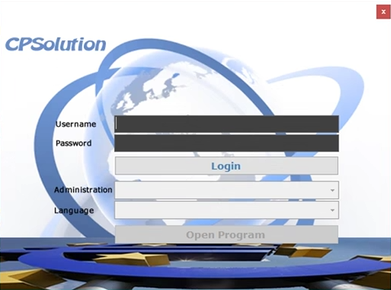
\includegraphics[]{img/erp/cpsolution.png}
	\caption{\label{fig:cpsolution}Aanmeldpagina van CPSolution}
\end{figure}

CPSolution ontstond niet meteen als een compleet ERP-pakket. In een eerste fase werd het louter ontwikkeld als uitbreiding op een reeds bestaand ordersysteem. Dat gebeurde op vraag van een klant in 2011. Als kaasproducent had de klant nood aan software om orders te plannen op de productielijn. Hun ordersysteem, Unit4 Multivers, bood die functionaliteit echter niet. Daarom werd de vraag gesteld aan 14IT om een oplossing op maat te ontwikkelen. Er werd software geschreven die de orders uit Unit4 Multivers kon ophalen, om vervolgens te plannen op de productielijn. 

Door alsmaar groeiende requirements werd het programma steeds uitgebreid. Zo kon het na verloop van tijd rechtstreeks gebruikt worden voor de opname van orders. Er werden modules toegevoegd om facturen en creditnota op te maken. Zo was ook de link naar een extern boekhoudsysteem niet meer nodig. Door dergelijke uitbreidingen groeide het programma meer en meer uit tot een autonoom ERP-systeem. In 2014 werd besloten om van hieruit een nieuw softwareproject op te starten onder de naam CPSolution.

\section{Dataopslag}
\label{sec:dataopslag}

\subsection{Type databank}
\label{sub:type-databank}

De data van het ERP-systeem wordt opgeslagen in een relationele databank van Microsoft SQL Server. De gebruikte editie is afhankelijk van de grootte en de noden van de klant. Voor kleine bedrijven volstaat een Express-editie soms al. Voor klanten zoals Lumap, die maandelijks honderden facturen te verwerken krijgen, is een Enterprise editie aangewezen. Onderstaande tabel is een greep uit de Microsoft documentatie om een beeld te geven van deze edities.

\begin{table}[H]
	\centering
	\begin{tabular}{@{}lccc@{}}
		\cmidrule(l){2-4}
		Maximum ...                                                                           & \textbf{Express}                                                         & \textbf{Standard}                                                          & \textbf{Enterprise} \\ \midrule
		\begin{tabular}[c]{@{}l@{}}compute capacity \\ used by a single instance\end{tabular} & \begin{tabular}[c]{@{}c@{}}lesser of 1 socket \\ or 4 cores\end{tabular} & \begin{tabular}[c]{@{}c@{}}lesser of 4 sockets\\  or 24 cores\end{tabular} & OS maximum          \\ \midrule
		\begin{tabular}[c]{@{}l@{}}memory for buffer \\ pool per instance\end{tabular}        & 1410 MB                                                                  & 128 GB                                                                     & OS maximum          \\ \midrule
		\begin{tabular}[c]{@{}l@{}}memory-optimized \\ data size per database\end{tabular}    & 352 MB                                                                   & 32 GB                                                                      & unlimited           \\ \midrule
		relational database size                                                              & 10 GB                                                                    & 524 PB                                                                     & 524 PB              \\ \bottomrule
	\end{tabular}
	\caption{\label{tab:sql-server-edities}Vergelijking van Microsoft SQL Server 2019 edities}
\end{table}


\subsection{Hosting}
\label{sub:hosting}

Naast de editie van de databank is ook de hosting van belang. Voor het ontwikkelen van CPSolution laat 14IT een databank hosten door Combell. In gebruik hebben klanten drie keuzes voor de fysieke opslag van deze databank:

\begin{itemize}
	\item \textbf{On-premises:} De databank wordt opgeslagen op een toestel in het intern netwerk van de klant. Indien nodig installeert 14IT hiervoor de nodige hardware. Deze optie vraagt dus een zekere investering van de klant, maar heeft als voordeel dat de data heel snel raadpleegbaar is.
	\item \textbf{Combell-hosting:} Er wordt beroep gedaan op een van de databasepaketten van Combell. Aangezien de software lokaal bij de klant geïnstalleerd wordt, dient men rekening te houden met een zekere latentie.
	\item \textbf{CPSolution on Cloud:} De databank en software worden opgeslagen op een fysiek toestel van 14IT dat instaat als server. Om de toepassing te delen met de klant bestaan twee mogelijkheden. Ofwel opteert de klant voor een published application. De klant zal lokaal een applicatie kunnen openen. Hoewel het lijkt alsof de applicatie lokaal draait, wordt er achterliggend eigenlijk een sessie op de server gestart. Enkele klanten maken gebruik van remote desktop om zo te interageren met het toestel.
\end{itemize}

\subsection{Datamodel}
\label{sub:datamodel}

De databank van CPSolution is opgebouwd volgens een relationeel model. Het model begon kleinschalig, maar groeide uit tot een enorm netwerk van tabellen. Dat gebeurde naargelang er nieuwe requirements kwamen van klanten. Momenteel is het datamodel zodanig uitgebreid dat het vrijwel niet op papier voor te stellen valt. Onderstaande afbeelding is slechts een deel van het ERD. Dat geeft al een idee van de omvang van de databank.

\begin{figure}[H]
	\centering
	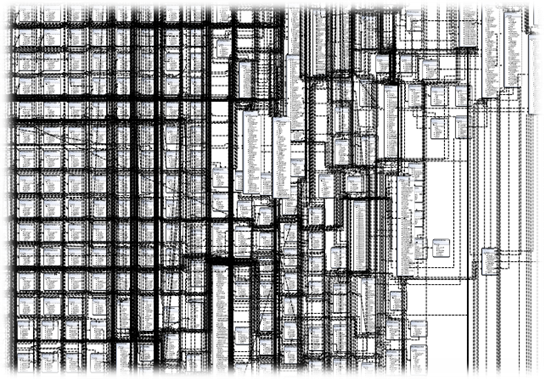
\includegraphics[]{img/erp/cpsolution-dbml.png}
	\caption{\label{fig:cpsolution-dbml}Blik op het datamodel van CPSolution}
\end{figure}


Om orde aan te brengen in het enorme aantal tabellen, werkt 14IT met een vaste naamgeving.
Tabellen die conceptueel rond eenzelfde thema draaien, worden voorafgegaan door eenzelfde afkorting. Op die manier worden de tabellen onderverdeeld in subcategorieën die van elkaar gescheiden worden met een onderstrepingsteken. Alle tabellen inzake producten worden bijvoorbeeld voorafgegaan door de aanduiding \verb*|PROD_|. Bepaalde subgroepen van de producttabellen kunnen nog verder gegroepeerd worden. Tabellen die beginnen met \verb*|CPS_PROD_PA_| zijn daar een voorbeeld van. Ze betreffen de ``PurchaseAgreements'' van producten. 

\begin{figure}[H]
	\centering
	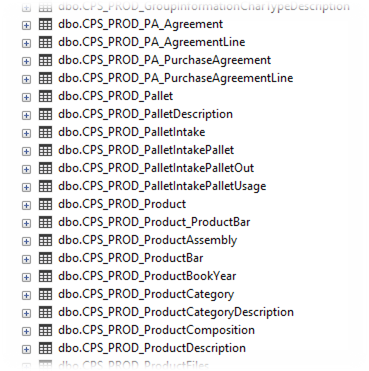
\includegraphics[width=0.5\linewidth]{img/erp/naamgeving-tabellen.png}
	\caption{\label{fig:naamgeving-tabellen}Naamgeving van tabellen}
\end{figure}

De databank van CPSolution kent een heel aantal prefixen. Deze hangen vaak samen met een bepaalde module. Aangezien een lijst met modules~\footnote{Zie bijlage} iets bevattelijker is, is het niet nodig om al deze prefixen ook op te lijsten.

Enkele bijzondere tabellen zijn die met prefix:
\begin{itemize}
	\item \verb*|IMP_|: Deze tabellen dienen als tussenstap om data uit Excel-bestanden van een klant te importeren in de databank. In deze tussenstap kan gecontroleerd worden of de data compleet en consistent is. Daarna kan men op basis van deze tabel kiezen welke rijen al dan niet geïmporteerd moeten worden. Dan gaat die data van de \verb*|IMP|-tabel naar zijn \verb*|CPS|-equivalent.
	\item \verb*|BCK_|: De tabellen die gebruikt worden om back-ups van de data te voorzien.
	\item \verb*|ERR_|: Een tabel die errors en logs van het systeem bijhoudt.
	\item \verb*|LOGS_|: Lijst van logins met gebruikersnaam en tijdstip.
	\item \verb*|X_|: Wanneer klanten specifieke databehoeften hebben, is er soms nood aan een tabel die enkel voor die klant gebruikt zal worden. Die krijgen deze aanduiding.
	\item \verb*|MON_|: 14IT kan indien gewenst allerlei processen bij de klant monitoren. Zo kan men bijvoorbeeld nagaan of er een probleem is met de automatische back-ups. Hiervoor wordt op geregelde tijdstippen data opgeslagen in de \verb*|MON|-tabellen. 
\end{itemize}

Tabellen met het achtervoegsel ``Discription'' houden de vertalingen bij van een specifieke tabel. Zo worden de vertalingen voor de records in CPS\_PROD\_Product bijgehouden in de tabel \verb*|CPS_PROD_ProductDescription|. Standaard worden de talen Engels, Frans en Nederlands voorzien. Klanten kunnen echter ook een extra module aanvragen om zelf extra vertalingen te voorzien in een andere taal zoals het Pools.

Wanneer een klant een nieuwe requirement stelt voor het ERP-systeem, wordt vanuit ontwikkeling steeds bekeken of het praktijkprobleem van dat bedrijf kan veralgemeend worden naar een module die voor meerdere klanten interessant is. Zulke uitbreidingen of wijzigingen vereisen soms een zekere datarefactoring. Het ontwerp van de databank wordt dan aangepast, met als doel een zo generiek mogelijk systeem te ondersteunen. 


\section{Electronic data interchange}
\label{sec:electronic-data-interchange}
Sinds de digitale revolutie is het gangbaar geworden om bedrijfsdocumenten zoals facturen, orders en rekeningen elektronisch uit te wisselen. Dit gegeven kreeg de algemene term ``electronic data interchange'' (EDI) toegeschreven. 
EDI biedt als voordeel dat het ontvangende bedrijf het document efficiënter kan opnemen in een eigen digitaal systeem. Een fysiek document, daarentegen, vereist daarvoor manuele ingave of geavanceerde technieken zoals OCR~\footnote{Optical character recognition software kan gebruikt worden om tekst te extraheren uit een afbeelding.}. Desondanks blijven ook deze papieren varianten een vaste waarde in het bedrijfsleven.

\subsection{Moeilijkheden}

Het hele EDI-gebeuren vereist dat de interne systemen van onderhandelende partijen op elkaar afgestemd zijn. Voor software-ontwikkelaars is dit geen evidente opdracht. 

\subsubsection{Aaneenschakeling}
Een deel van dit probleem probeerde men te vereenvoudigen door vaste EDI-standaarden af te spreken. Ondernemingen kunnen dan de nodige ``vertalingen'' voorzien van hun data naar het gedeelde formaat, in plaats van een rechtstreekse omzetting te moeten maken naar het externe systeem. Dergelijke omzettingen, veroozaken weinig problemen indien het een enkele overschakeling betreft. Binnen een context van een supply chain, waar factuurdata doorheen verschillende ondernemingen moet gaan, kan een veelvoud van ``vertalingen'' er echter voor zorgen dat de benodigde, correcte data verloren gaat. Als analogie kan men dit probleem vergelijken met het spelletje ``Chinees gefluister''\footnote{Chinees gefluister is de titel van een spelletje waarin kinderen op een rij staan, met als doel een boodschap van persoon tot persoon door te fluisteren. Vaak probeert men met dit spelletje de kinderen te laten ondervinden dat de boodschap drastisch veranderd kan zijn, op het moment dat het bij de laatste schakel aankomt.}. In een ideaal scenario zou de oorsponkelijke data van elke stap in de schakel steeds beschikbaar moeten blijven.


\subsubsection{Confidentialiteit}
Daarnaast is het ook belangrijk dat de data de juiste ontvanger bereikt. Data over de onderhandelingen tussen twee ondernemingen moeten niet openbaar zijn, maar moeten tegelijk wel steeds op een vlotte manier raadpleegbaar zijn voor beide partijen.

\subsubsection{Verifieerbaarheid}

In de andere richting moet de ontvanger ook kunnen verifiëren dat de data van de juiste partij afkomstig is. In de praktijk gaat dit doorgaans gepaard met manuele checks op basis van papieren facturen. Daarnaast moet ook nog de digitale versie van de factuur nagekeken worden. Dat zorgt voor heel wat dubbelwerk. 


\subsection{As is}
CPSolution staat niet rechtstreeks in contact met andere systemen om aan EDI te doen. Hiervoor wordt beroep gedaan op de services van Basware. Bestanden zoals orders en facturen worden als een gestructureerde XML naar BasWare gestuurd. Zij vormen het om naar het juiste EDI formaat en sturen dit door naar de ontvanger.


Bedrijven hebben hun eigen systemen die niet altijd op elkaar zijn afgestemd qua dataoverdracht. Om dit probleem aan te pakken, werden EDI-standaarden afgesproken. Bedrijven kunnen zich dan afstemmen om deze formaten, om de data te vertalen naar een formaat dat binnen hun ERP-pakket past.

CPSolution staat niet rechtstreeks met andere systemen in contact om aan EDI te doen. Hiervoor wordt beroep gedaan op de services van Basware. Bestanden zoals orders en facturen worden als een gestructureerde XML naar BasWare gestuurd. Zij vormen het om naar het juiste EDI formaat en sturen dit door naar de ontvanger.


\chapter{Blockchaintoepassingen voor ERP}
\label{ch:blockchaintoepassingen-voor-erp}

Dit hoofdstuk slaat de brug tussen de twee voorgaande deelvragen. Het representeert de zoektocht naar die blockchaintechnologieën die bruikbaar zijn binnen een ERP-context. Het gaat dus over de derde deelvraag van het onderzoek:

\begin{center}
	\textit{\textbf{``Welke mogelijkheden bieden blockchains voor een ERP-systeem?''}}
\end{center}

Om die mogelijkheden te vinden, werd vertokken vanuit de Gartner Hype Cycle uit Sectie \ref{sec:verantwoording} - \nameref{sec:verantwoording}. De toepassingen blockchainplatform en \textit{smart contract} komen om die reden als eerste aan bod.

De eerste sectie geeft een inzicht in de verschillende varianten aan blockchains. Elk platform werd ontwikkeld volgens eigen ontwerpkeuzes. Als gevolg hebben ze niet allemaal hetzelfde toepassingsgebied.

De volgende sectie maakt duidelijk dat er ook scripts of programmatuur op een blockchain gebracht kunnen worden. Deze \textit{smart contracts} bieden allerlei nieuwe mogelijkheden zoals NFT's. 

Om de overstap naar de laatste deelvraag te maken, werd een laatste sectie toegeweid aan NFT's. Een concreet voorbeeld illustreert dat het mogelijk is om allerlei data in een blockchain op te nemen. Daarmee wordt een conceptuele sprong gemaakt die absoluut nodig was om de proof of concept op poten te zetten.

\section{Blockchainplatformen}

De originele \textit{Bitcoin} \textit{whitepaper} inspireerde talloze spelers om een eigen versie van een blokchain te ontwikkelen. Ondertussen brachten al verschillende ondernemingen hun eigen variant op de markt. Om deze implementaties van elkaar te onderscheiden spreekt men over verschillende ``blockchainplatformen''. Elk platform biedt een basis aan ontwikkelaars om nieuwe toepassingen te bouwen op de bestaande blokchain-infrastructuur
~\autocite{Saraf2018}.

\begin{table}[H]
	\begin{tabular}{@{}lccc@{}}
		\cmidrule(l){2-4}
		& \textbf{Ethereum}                                         & \textbf{Hyperledger} & \textbf{R3 Corda}                                        \\ \midrule
		1. Type                                                                     & Openbaar                                                  & Besloten             & Besloten                                                 \\ \midrule
		2. Consensus algoritme                                                      & Proof of Work                                             & Pluggable Framework  & Pluggable Framework                                      \\ \midrule
		3. Toepassingsgebied                                                        & Algemeen                                                  & Algemeen             & Financiële sector                                        \\ \midrule
		\begin{tabular}[c]{@{}l@{}}4. Ondersteunde\\  programmeertalen\end{tabular} & \begin{tabular}[c]{@{}c@{}}Python\\ Go\\ C++\end{tabular} & Python               & \begin{tabular}[c]{@{}c@{}}C++\\ Javascript\end{tabular} \\ \bottomrule
	\end{tabular}
	\caption{\label{tab:blockchainplatformen}Vergelijking van drie fundamentele blockchain platformen}
\end{table}

Een eerste manier waarop platformen zich van elkaar onderscheiden is de programmeertaal waarin ze geïmplementeerd zijn.
Tabel~\ref{tab:blockchainplatformen} vergelijkt drie fundamentele blockchainplatformen met elkaar op nog een aantal andere vlakken.

\begin{enumerate}
	\item Een platform kan openbaar of besloten zijn. Indien men geen permissies nodig heeft om het peer-to-peernetwerk te betreden, wordt het als openbaar beschouwd. In het andere geval is het systeem besloten. Eens een node opgevangen is in het netwerk, kan het de blockchain in beide op een transparante manier inkijken.
	\item Niet elk platform gebruikt de Proof of Work, zoals beschreven in sectie \ref{sub:proof-of-work} - \nameref{sub:proof-of-work}. Er zijn ook andere manieren om consensus na te streven. Het opzet blijft echter hetzelfde.
	\item Verschillende platformen mikken op een ander toepassingsgebied.
	\item Naast de taal waarin de blockchain geïmplementeerd is, zijn er ook programmeertalen waarmee het platform benaderd kan worden. Hiermee kunnen ontwikkelaars toepassingen schrijven die de onderliggende blockchain kunnen benutten. 
\end{enumerate}
	
\pagebreak
	
Deze drie voorbeelden werden opgenomen in de tabel, omdat ze in zekere zin een basis vormen van vele andere platformen. Heel wat producenten brachten een eigen platform op de markt dat eigenlijk een afgeleide is van reeds bestaande keuze. In de literatuur wordt vaak geen onderscheid gemaakt tussen de twee~\autocite{Gartner2022}. Enkele voorbeelden van commerciële blockchainplatformen zijn:
\begin{itemize}
	\item Ethereum
	\item Hyperledger Fabric
	\item Hyperledger Sawtooth
	\item Hyperledger Iroha
	\item IBM Blockchain
	\item Microsoft Azure Blockchain
	\item ...
\end{itemize}

\subsection{Hard forks}

Zoals reeds vermeld, kunnen blockchainplatformen de basis vormen voor nieuwe varianten. Wanneer er ingrijpende aanpassingen gemaakt worden aan het protocol van een basis-blockchain, spreekt men over een ``hard fork''. Door uiteenlopende visies kunnen op die manier verschillende ``smaken'' van eenzelfde blockchain ontstaan. Wanneer men over de Bitcoin-blockchain spreekt, heeft men het doorgaans over de originele BTC-fork. Nochtans is dit niet de enige. Sinds het ontstaan werd er steeds verder getweakt aan de implementatie. Omdat informatici een eigen visie hadden over hoe de keten stabiel gemaakt kon worden, ontstonden ook forks zoals BSV (Blockchain Satoshi Vision). In die vertakking probeerde men zoveel mogelijk terug te keren op het oorspronkelijk protocol. Verschillende ontwerpkeuzes zorgen ervoor dat de ene fork meer schaalbaarheid of rekenkracht kan bieden dan de andere. Als gevolg zijn bepaalde forks meer of minder geschikt voor het opslaan van data in een ERP-context.

\section{Smart contracts}

Een \textit{smart contract} is een stuk computercode dat geïmplementeerd wordt bovenop een blockchain als digitale versie van een contract. Ze maken het mogelijk om contractuele voorwaarden automatisch af te dwingen, zonder de tussenkomst van een derde partij~\autocite{Salem2008}.

De voorwaarden en bijhorende gevolgen van het contract, worden omgezet naar verzameling van functies en variabelen in het \textit{smart contract}. Wanneer transacties in de blockchain terecht komen die een van deze voorwaarden triggert, wordt de bijhorende functie uitgevoerd. De uitvoer wordt op zijn beurt opgenomen in de blockchain als een nieuwe transactie~\autocite{Zheng2019}. In volgende subsecties worden de verschillende stappen in de levenscyclus van een \textit{smart contract} uitgelegd. Figuur~\ref{fig:smart-contracts-overview} geeft een mooie leidraad weer.

\begin{figure}[]
	\centering
	\includegraphics[width=\linewidth]{img/blockchaintoepassingen-voor-erp/smart-contracts-overview.pdf}
	\caption{\label{fig:smart-contracts-overview}Overzicht \textit{smart contracts}~\autocite{Zheng2019}}
\end{figure}

\subsection{Creatie}

In een eerste fase leggen de betrokken partijen de voorwaarden van het contract vast in gewone mensentaal. Eens opgesteld, kan een software engineer de (voorwaarden van) dit contract omzetten in code. Dit is mogelijk in verschillende high-level programmeertalen, zoals Python, Java of Solidity~\autocite{Bahga2016}. Een compiler zet deze statements om naar een \textit{smart contract} onder de vorm machinecode, dat klaar is om in de blockchain gezet te worden~\autocite{Zheng2019}.

\textbf{Voorbeeld:}
Partijen A en B sluiten een contract: indien een metaaldetector iets aantreft in de voedselverwerking van partij A, moet partij B hiervoor beboet worden. Een software engineer krijgt de opdracht om dit contract om te zetten in code.

\subsection{Deployment}

Eens een contract wordt weggeschreven naar de blockchain, kan het niet meer gewijzigd worden. Zoals al aangegeven, zijn de voorwaarden van het contract vertaald naar functies en variabelen. Indien men een nieuwe voorwaarde wenst toe te voegen aan het contract, zal men een nieuw \textit{smart contract} moeten aanmaken. Dankzij de transparantie van de blockchain kunnen alle partijen het contract raadplegen~\autocite{Zheng2019}.

\textbf{Voorbeeld:}
Het \textit{smart contract} tussen partij A en B wordt op de blockchain geplaatst.

\subsection{Uitvoering}

Tijdens de uitvoering wordt voortdurend gemonitord of er nieuwe transacties op de blockchain geplaatst worden die de voorwaarden van het contract vervullen. Wanneer een functie getriggerd word zal deze de voorgeprogrammeerde implicaties uitvoeren als een nieuwe transactie in de blockchain. Met andere woorden: het contract werd afgedwongen, zonder actieve tussenkomst van een derde partij~\autocite{Delmolino2016}.

\textbf{Voorbeeld:}
De metaaldetector van partij A merkt een onzuiverheid op in het productieproces. Deze detectie wordt onder de vorm van een transactie opgeslagen op de blockchain. Dit triggert het \textit{smart contract} dat op zijn beurt een transactie op de keten plaatst om aan om deze gebeurtenis te documenteren.

\subsection{Afronding}

Om de levenscyclus van een \textit{smart contract} af te ronden, worden de betrokken partijen op de hoogte gebracht. De status van de partijen wordt geüpdatet indien nodig~\autocite{Zheng2019}.

\textbf{Voorbeeld:}
Partijen A en B worden op de hoogte gebracht. Partij B maakt het nodige bedrag over naar partij A, wat wordt geregistreerd als een transactie op de blockchain.



\section{NFT's}

Zoals vermeld in Subsectie \ref{sub:transacties} - \nameref{sub:transacties}, stond een transactie oorspronkelijk voor de bitcoin-overdracht van een partij naar een andere~\autocite{Pierro2017}. Bij elke transactie worden digitale tokens uitgewisseld die door de ontvangende partij opnieuw uitgegeven kunnen worden. Op geen enkel punt is het daarbij zinvol om een onderscheid te maken tussen individuele tokens. Ze zijn namelijk onderling gelijkwaardig. Zo komt een Bitcoin wallet aan zijn saldo lauter door het aantal bitcoins waaruit het bestaat. Het is daarbij niet van belang wélke bitcoin-tokens dat specifiek zijn. In die zin zijn de tokens van Blockchain 1.0 fungibel of vervangbaar.

Met de overgang naar Blockchain 2.0 wordt op dit vlak een conceptuele sprong gemaakt. Met de komst van nieuwe blockchainplatformen werd het namelijk mogelijk om meer dan enkel bitcoin-overdrachten op te slaan. De datavelden van nieuwere blockchains staan open voor allerlei data. Men kan nu ook bestanden zoals een afbeelding, factuur of tekstbestand vastleggen in een blockchain en behandelen als een token. Deze tokens kunnen nog steeds uitgewisseld worden, maar hebben nu wel een unieke waarde. Immers, de ene factuur is de andere niet. Ze zijn dus niet fungibel en krijgen daarom de naam Non-fungible token of NFT.

Een diepgaande technische uiteenzetting van NFT's is niet opportuun voor deze scriptie. Aangezien deze tokens wel hun nut bewijzen in een ERP-context, is het echter wel belangrijk om een gegrond beeld te krijgen van wat ze juist zijn.

\subsection{Voorbeeld}

Op digitale markplaatsen zoals OpenSea kan men de inhoud en details van allerlei NFT's verkennen. Deze bevinden zich op een blockchain zoals die van Ethereum. Heel wat grafische kunstwerkjes worden op die manier ``als NFT'' te koop aangeboden. Onderstaand voorbeeld illustreert wat dat juist inhoudt.

Figuur~\ref{fig:nft-example} geeft een willekeurige NFT uit de Ethereum blockchain weer, zoals die te vinden valt op digitale markplaatsen. De data die in dit geval als token op de blockchain geplaatst werd, is een PNG-afbeelding van cirkels en lijnstukken. Het is belangrijk om erop te wijzen dat dit geen afbeelding hoeft te zijn. Ook andere bestanden, zoals een XML-factuur of een mp3 zijn mogelijk. In de details wordt verwezen naar het \textit{smart contract} waarmee deze token gemaakt werd, alsook de ID dat eraan gegeven werd.

\begin{figure}[H]
	\centering
	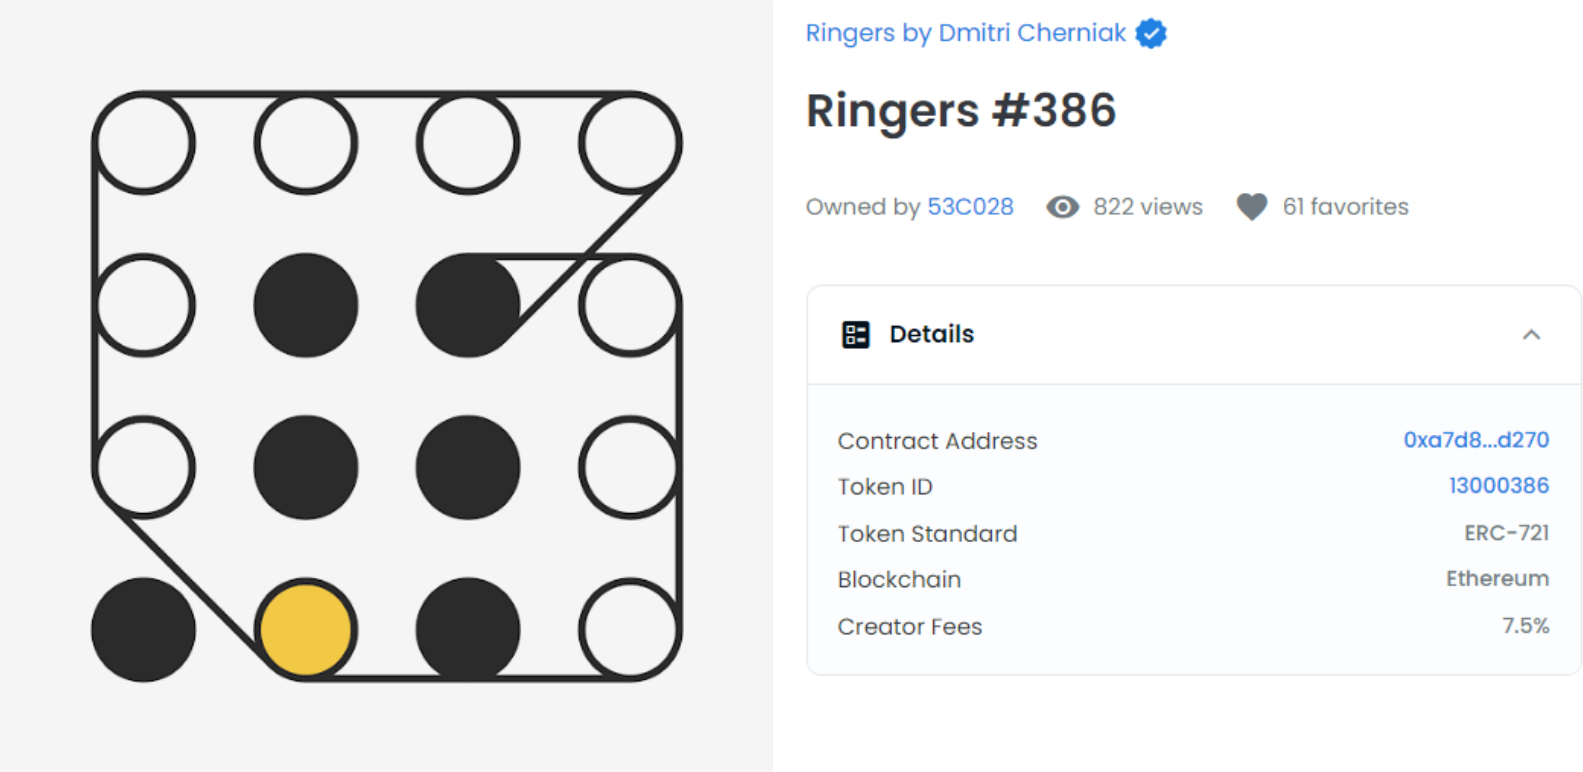
\includegraphics[width=\linewidth]{img/blockchaintoepassingen-voor-erp/nft-example.png}
	\caption{\label{fig:nft-example}NFT op een digitale marktplaats}
\end{figure}

Het \textit{smart contract} adres wijst naar een plaats op de Ethereum blockchain. Een eenvoudige manier om de bijhorende data te benaderen, is met behulp van een block explorer website zoals EtherScan. Wie het adres volgt, zal het script (of \textit{smart contract}) vinden dat gebruikt werd om de afbeelding, samen met allerlei metadata op de blockchain te plaatsen. Met andere woorden: het werd gebruikt om de afbeelding ``als NFT'' op de blockchain te plaatsen. Hiervoor heeft het script allerlei commando's. Nog een ander commando dient ervoor om de URI van een token op te vragen op basis van zijn ID:
\begin{figure}[H]
	\centering
	\includegraphics[width=\linewidth]{img/blockchaintoepassingen-voor-erp/tokenURI-function.pdf}
\end{figure}
Met de ID van de NFT uit Figuur~\ref{fig:nft-example} als parameter, zal dit commando kunnen we de bijhorende URI retourneren.

\begin{figure}[H]
	\centering
	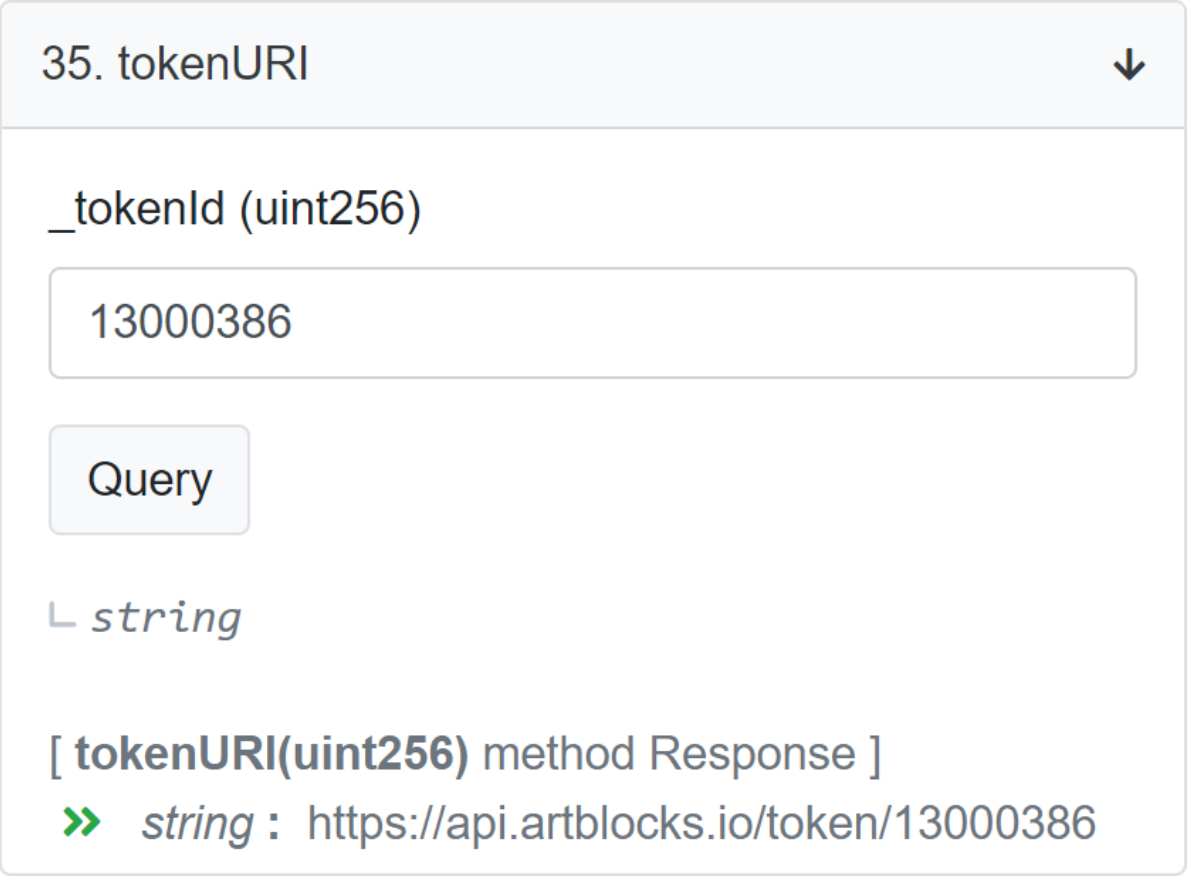
\includegraphics[width=0.5\linewidth]{img/blockchaintoepassingen-voor-erp/nft-tokenURI.png}
	\caption{\label{fig:nft-tokenURI}URI van een NFT}
\end{figure}

Merk op dat de token URI in dit geval zelfs een URL is. Deze kan dus via elke webbrowser benaderd worden. Het is trouwens ook mogelijk om dit adres als QR-code voor te stellen. Door deze verwijzing te volgen, krijgt men de data van de NFT\footnote{Voor de duidelijkheid werd een deel van de metadata uit dit voorbeeld vervangen door beletseltekens.}:

\begin{figure}[H]
	\centering
	\includegraphics[width=\linewidth]{img/blockchaintoepassingen-voor-erp/NFT-data.pdf}
\end{figure}

De NFT bestaat uit metadata zoals \verb|tokenID|, \verb*|payout_address| en \verb|minted|. Met \verb*|image| wordt de URI-verwijzing naar de PNG-afbeelding van cirkels vastgelegd. Het geheel is wat ``de NFT van'' de afbeelding inhoudt. 
Wat het betekent om een NFT van een bestand te minten kan dus eenvoudig beschreven worden: men plaatst -met behulp van een \textit{smart contract}- een URI-verwijzing naar dat bestand, samen met metadata op de blockchain. Die data geniet vanaf dan alle voordelen van een blockchain: het is \textit{incorruptible} en kan herleid worden naar een zekere eigenaar.

\chapter{Proof of concept}
\label{ch:proof-of-concept}



In dit hoofdstuk werd getracht om, steundend op een proof of concept, een antwoord te bieden op de laatste deelvraag van het onderzoek:

\begin{center}
	\textit{\textbf{``Hoe kunnen softwareontwikkelaars de data van het ERP-systeem opslaan in een blockchain?''}}
\end{center}

Het opzet van deze proof of concept, was in eerste instantie om aan te tonen dat het effectief gelukt is om data op te slaan in een blockchain. Hiervoor werd gebruik gemaakt van de services van mintBlue. Daarenboven wordt met deze proof of concept ook de aanzet gegeven tot een echte use case voor dit gegeven: NFT invoicing. Tot slot wordt ook een schets gemaakt van het kostenplaatje dat hierbij komt kijken. Het hoofdstuk eindigt met een kritische noot.


\section{Data op de blockchain plaatsen}
\label{sec:data-op-de-blockchain-plaatsen}

Zoals al vermeld in Sectie \ref{sec:nfts} -- \nameref{sec:nfts} is het mogelijk om eender welke data op te nemen in een blockchain. In deze sectie staat beschreven hoe data uit het ERP-systeem op de blockchain geplaatst kan worden. Meer bepaald de data van een digitale factuur.

\subsection{Digitale facturen}
\label{sub:digitale-facturen}

Zoals kort aangehaald in Sectie \ref{sec:enterprise-resource-planning} -- \nameref{sec:enterprise-resource-planning} zijn er verschillende manieren om facturen digitaal op te slaan en uit te wisselen.
Bij voorkeur wordt hiervoor een bestand gebruikt dat de data van die factuur op een gestructureerde manier bijhoudt. Dergelijke bestanden worden ook wel e-invoices genoemd. Hiervoor bestaan een aantal gangbare formaten zoals EDI, XML of CSV. Als bestuurslid van werkgroep UBL.BE\footnote{UBL.BE werd opgericht met als doel het gebruik van elektronische documenten in kmo's te bevorderen. De vereniging zet in op UBL-standaarden om uitwisseling van documenten tussen ondernemingen te vergemakkelijken.}, maakt 14IT gebruik van XML-bestanden. Deze worden opgebouwd volgens syntax en regels die werden vastgelegd in de UBL-standaard. Daarom noemt men dit ook, kortweg, UBL-bestanden. Onder die vorm, is een e-invoice in se een tekstbestand waarin factuurgegevens genoteerd staan aan de hand van vastgelegde XML-tags. Het adres van de klant zou hierin bijvoorbeeld als volgt kunnen voorkomen:

\begin{figure}[H]
	\centering
	\includegraphics[width=\linewidth]{img/proof-of-concept/xml-example.pdf}
\end{figure}


\subsection{Data wegschrijven}
\label{sub:data-wegschrijven}

Aangezien digitale facturen niet meer zijn dan een gestructureerd XML-bestand, kunnen ze als NFT gemint worden. Dat betekent dat er een ``transactie'' met (verwijzing naar) de factuur op de blockchain geplaatst kan worden. Om dit principe aan te tonen, werd -in het licht van dit onderzoek- een mock-factuur opgesteld. Het bestand werd in \href{https://whatsonchain.com/tx/71054b6b9aef47124cc5db9983a06d7608ec408c1ed3ee3a0ad0e34e2951c83c}{\textcolor{blue}{transactie 710...83c}} op de BSV-blockchain gebracht. Figuur~\ref{fig:factuur-transactie} geeft de inhoud van de transactie weer, zoals deze te vinden is via een online \textit{block explorer}. Volgende paragrafen geven meer uitleg bij de details van deze transactie.

Op blok \#738410 van de BSV-blockchain bevindt zich een transactie die de mock-factuur van deze bachelorproef bevat. Een transactie is en blijft nog steeds een bitcoin-uitwisseling van input naar output. De bitcoin (in dit geval BSV) kunnen over meerdere outputs verdeeld worden. Het is zelfs mogelijk om outputs van 0 BSV op te nemen. Hier wordt handig gebruik van gemaakt om de data van de factuur op te slaan.

In ons voorbeeld werd een input van 0.00001968 BSV ``verdeeld'' over twee outputs. Om miners aan te moedigen deze transactie op te nemen in het blok, werd een fee betaald van 0.00000303 BSV. Het overblijvende bedrag gaat integraal naar output \#1. Dit stelt een uitwisseling voor van 0.00001665 BSV van en naar hetzelfde adres 1AT...uyy.

Output \#0 is een \textit{data-carrying} output. Het werd uitsluitend gecreëerd als vehicel voor de data van de factuur. Daarom gaat er 0 BSV naartoe en kent het tevens geen adres. De \verb|OP_RETURN| geeft aan dat dit over een output gaat die niet gespendeerd kan worden. In het bijhorende tekstveld zien we de voornaamste inhoud van deze output, namelijk de digitale factuur.

\begin{figure}[H]
	\centering
	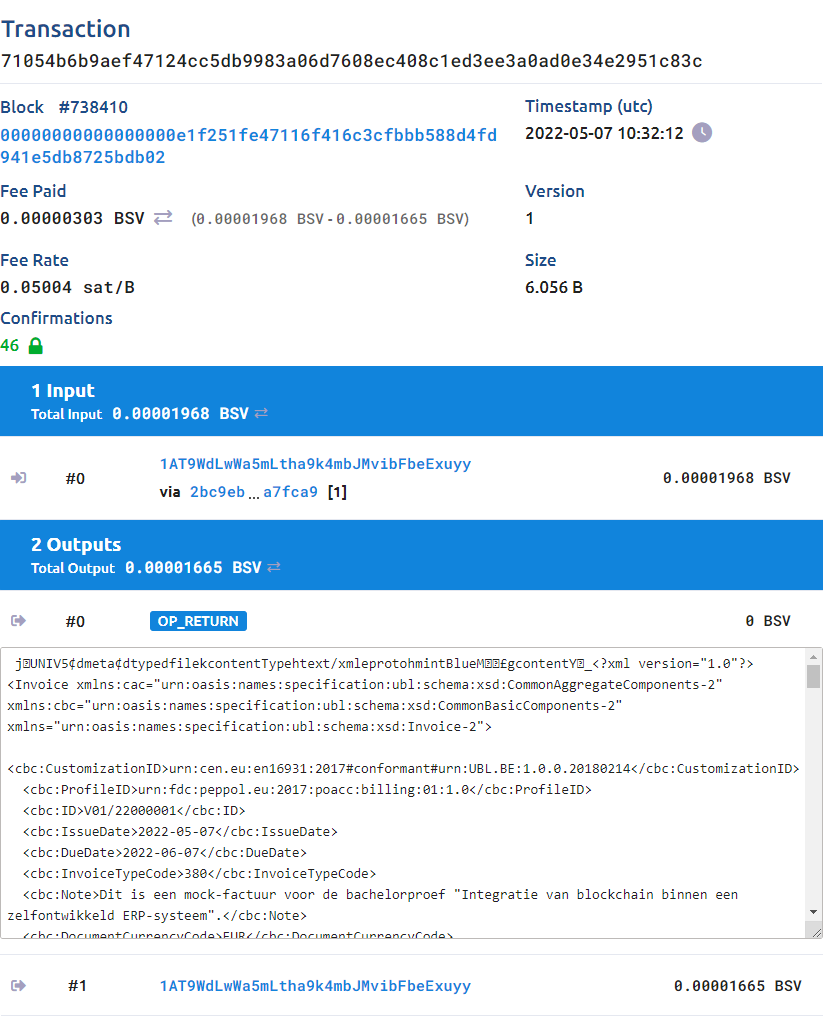
\includegraphics[width=\linewidth]{img/proof-of-concept/factuur-transactie.png}
	\caption{\label{fig:factuur-transactie}E-invoice als transactie op de BSV-blockchain}
\end{figure}

De e-invoice is vanaf nu dus definitief aanwezig als data op de BSV-blockchain. Kortom betekent dit dat de factuur digitaal beschikbaar is voor de ontvanger. Elke BSV-node kan ze opvragen via het \verb*|TXID| van de omvattende transactie. Het is echter geen vereiste om een eigen node op te zetten. Publieke API's zoals die van Blockchair maken het mogelijk om met een eenvoudige \href{https://api.blockchair.com/bitcoin-sv/raw/transaction/031fcc00b88fcc2252107be98c085eea528c470df9d910387947f60adae80287}{\textcolor{blue}{URL}} de ruwe data (JSON) van een transactie op te vragen. De factuur kan uitgelezen worden door de \verb*|hex|-waarde van \verb*|vout| \verb*|0| om te zetten naar ASCI. De \textit{block explorer} in Figuur~\ref{fig:factuur-transactie} doet dit automatisch.


\begin{figure}[H]
	\centering
	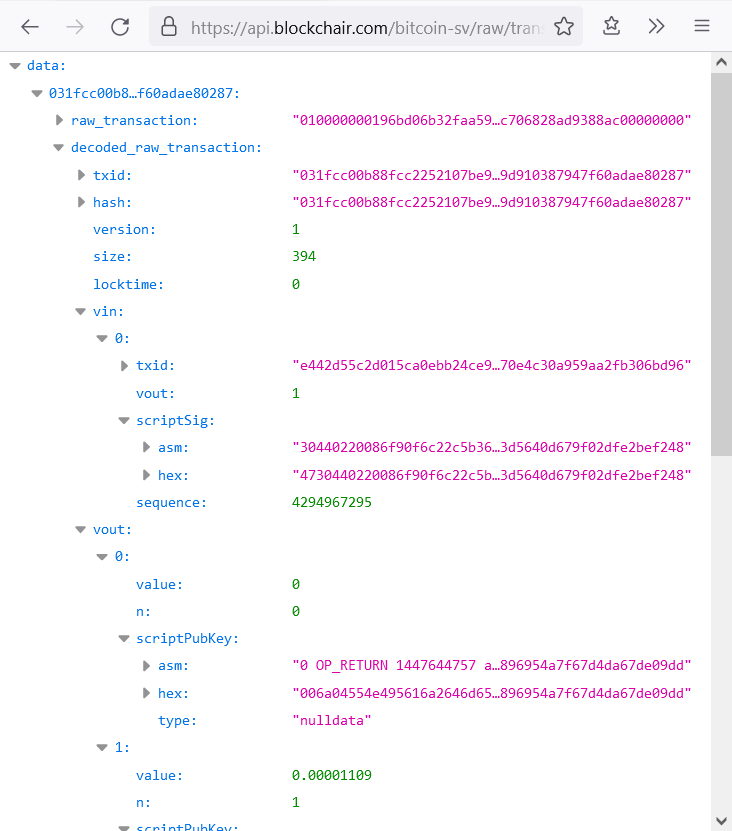
\includegraphics[width=0.8\linewidth]{img/proof-of-concept/ruwe-transactie.png}
	\caption{\label{fig:ruwe-transactie}Ruwe data van de transactie}
\end{figure}

\subsection{Encryptie}
\label{sub:encryptie}

Voorgaande subsectie toont aan dat het mogelijk is om de data van een digitale factuur op te slaan in een blockchain. Aangezien BSV een publieke blockchain is, is die factuur ook publiekelijk toegankelijk.

In plaats van de factuur rechtstreeks op de blockchain te plaatsen, zou het er ook geëncrypteerd opgeplaatst kunnen worden. Enkel partijen die beschikken over de \textit{encryption secret} zullen de data kunnen decrypteren en zo de factuur inkijken. 

\begin{figure}[H]
	\centering
	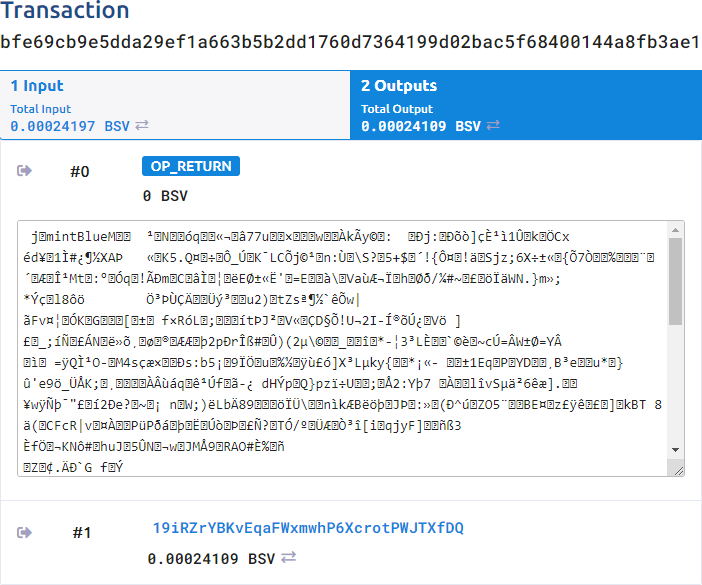
\includegraphics[width=\linewidth]{img/proof-of-concept/transactie-encryptie.png}
	\caption{\label{fig:transactie-encryptie}Transactie met geëncrypteerde e-invoice}
\end{figure}


\section{NFT invoicing}
\label{nft-invoicing}

Voorgaande sectie toont aan dat het mogelijk is om data uit het ERP-syteem op te slaan in een blockchain. De nodige encryptie zorgt ervoor dat enkel de bestemde partij ook toegang krijgt tot die data. Dit gegeven schept nieuwe mogelijkheden binnen het hele EDI-gebeuren.

\subsection{EDI-proces}
\label{sub:edi-proces}

Om de geëncrypteerde factuur uit Subsectie \ref{sub:encryptie} -- \nameref{sub:encryptie} uit te lezen, dient men de juiste transactie op te halen en vervolgens de \textit{data-carrying} output te decrypteren. Dit proces kan geprogrammeerd worden en afgeschermd alszijnde een API-methode. Deze vormt een endpoint die in het geval van een REST API zelfs met een URL kan aangeproken worden. De ontvanger kan de \verb|TXID| in combinatie met de \textit{encryption secret} dan gebruiken als token voor de digitale factuur.

Bovenstaand gegeven kan voor CPSolution concreet gebruikt worden voor een nieuw EDI-proces genaamd NFT invoicing.

Wanneer bedrijf A een factuur opstelt in CPSolution, wordt de bijhorende data opgeslagen in de SQL Server databank. Met behulp van een webservice wordt de factuur geëxtraheerd worden als UBL-bestand. Dit bestand wordt vervolgens geëncrypteerd op de blockchain geplaatst. Zo bekomt men een transactie zoals die in Figuur~\ref{fig:transactie-encryptie}. 

De factuur is vanaf dat moment immutable en staat klaar om opgehaald te worden. Ophalen kan -zoals hierboven reeds aangehaald- met een API-methode die op basis van de \verb|TXID| en \textit{encryption secret} de juiste transactie ophaalt en decrypteert. Vervolgens dient men, op basis van de \verb|TXID| en \textit{encryption secret} de juiste URL op te stellen om deze methode op te roepen. Deze URL kan op zijn beurt aangeboden worden onder de vorm van een QR-code. Het downloaden van de factuur herleidt zich dan tot het simpelweg scannen van deze code. Figuur~\ref{fig:qr-code} kan gescand worden om de mock-factuur uit Sectie \ref{sub:digitale-facturen} -- \nameref{sub:digitale-facturen} op te halen.

\begin{figure}[H]
	\centering
	
\includegraphics[width=0.25\linewidth]{img/proof-of-concept/qr-code.pdf}
	\caption{\label{fig:qr-code}QR-code om e-invoice op te halen van de BSV-blockchain}
\end{figure}

Op hetzelfde moment genereert CPSolution een pdf voor de fysieke factuur. Bijlage \ref{ch:mock-factuur} -- \nameref{ch:mock-factuur} is een voorbeeld van hoe deze papieren variant er zou kunnen uitzien. De QR-code wordt op dit fysieke document geplaatst. Daarmee bevat deze een verwijzing naar de bijhorende e-invoice, zoals die op de blockchain staat.

\begin{figure}[H]
	\centering
	\includegraphics[]{img/proof-of-concept/nft-invoicing.pdf}
	\caption{\label{fig:nft-invoicing}NFT invoicing}
\end{figure}

Bedrijf A zendt vervolgens deze fysieke factuur uit naar bedrijf B\footnote{Briefverkeer is vandaag de dag nog steeds een vaste waarde in het bedrijfsleven.}. Wanneer het personeel uit bedrijf B het document goedkeurt, kunnen ze de QR-code scannen. De e-invoice wordt automatisch gedownload en kan worden opgenomen in het eigen ERP-systeem of boekhoudpakket. 

\subsection{Voordelen}
\label{sub:voordelen}

NFT invoicing biedt als voordeel dat er steeds een referentie beschikbaar blijft naar de originele digitale versie van een factuur. Aangezien die versie op de blockchain staat, weet de ontvanger zeker dat deze ongewijzigd is. Het gedistribueerde en onvervalsbare karakter van de \textit{ledger} maken een ``\textit{single source of truth}'' mogelijk tussen meerdere onderhadelende partijen. Dit was een doel dat voorheen enkel nagestreefd werd binnen eenzelfde ERP-systeem\footnote{Zie Sectie \ref{sec:enterprise-resource-planning} -- \nameref{sec:enterprise-resource-planning}}. De immutability en transparantie van de blockchain zouden tevens allehande fraude zoals spookfacturen kunnen helpen tegengaan~\autocite{Sterk2021}. 

Anderzijds kan er met NFT-invoicing nog steeds voldaan worden aan de voorkeur van veel bedrijven om met fysieke documenten te werken. Om die papieren facturen op te nemen in het boekhoudsysteem, worden nu vaak OCR-technieken gebruikt. Dat is niet altijd evident aangezien de structuur van elk type factuur anders kan zijn. Daardoor moet de data telkens op een andere manier geïnterpreteerd worden door het boekhoudpakket. Door met een QR-code te werken, kan men vlot de originele digitale factuur ophalen. Deze kan veel vlotter ``overgegoten'' worden in een digitaal systeem aangezien het opgebouwd is volgens de UBL-standaard. Er moet dus maar een vertaling van UBL naar het eigen systeem voorzien worden, in plaats van een aparte vertaling voor elk type factuur.

\section{mintBlue}
\label{sec:mintBlue}

Softwarebedrijf mintBlue beweert het eerste publieke blockchain platform van Europa aan te bieden dat op grote schaal gebruikt kan worden. Het bedrijf, met vestigingen in Amsterdam en Antwerpen, ontwikkelt een API waarmee ontwikkelaars data kunnen opnemen in een blockchain. De infrastructuur steunt op de BSV-blockchain. In die zin biedt mintBlue zelf geen platform, maar wel een Blockchain PaaS. Vaak spreekt men simpelweg over Blockchain as a service. De naam ``mintBlue'' wordt uitwisselbaar gebruikt voor zowel het bedrijf als de service die ze bieden.

Het doel van mintBlue is om ontwikkelaars een gebruiksvriendelijke manier te bieden om lees- en schrijfoperaties van en naar de blockchain uit te voeren. Hiervoor bieden ze een API en SDK. Met behulp van deze service zou 14IT blockchain kunnen integreren in CPSolution, zonder eigen nodes of andere infrastructuur op te zetten of te onderhouden.

De services van mintBlue bevinden zich momenteel nog in een ontwikkelfase, waardoor ze nog niet publiekelijk beschikbaar zijn. Er is wel al een solide basis aanwezig. In het kader van deze bachelorproef werd vroegtijdige toegang tot het platform verleend.

\subsection{API}
\label{sub:api}

Met een API probeert mintBlue de complexiteit van een blockchain af te schermen. In eerste instantie voorziet deze POST- en GET-methodes voor transacties. Een ontwikkelaar kan dus snel een ``Write'' of ``Retrieve'' van een transactie naar de blockchain uitvoeren.

Daarnaast specifieert de API ook een aantal methodes om gebruik van het platform te ondersteunen, of om wisselwerking met Zapier\footnote{Zapier is een automatisatietool waarmee output van van een toepassing zoals e-mail of Google Drive kunnen gebruikt worden als trigger voor input in bijvoorbeeld de mintBlue-integratie. Op die manier kan men bijvoorbeeld een Zapier-proces definiëren dat bij het ontvangen van specifieke mails een bijhorende transactie op de blockchain plaatst. Deze intragaties werden niet gebruikt bij deze bachelorproef.} mogelijk te maken.

Een interessante deelverzameling is de Token API. Deze stelt developers in staat om volledige bestanden, zoals facturen of kredietnota, als NFT op de blockchain te plaatsen. De bestanden worden standaard geëncrypteerd, zodat ze enkel geraadpleegd kunnen worden met behulp van een referentie en secret.

Een eenvoudige manier om de API te benaderen, is met de mintBlue SDK. Voorlopig bestaat er enkel een SDK voor JavaScript. De bedoeling is dat er ook SDK's voor Elixir, Ruby en PHP ontwikkeld worden.

\subsection{Platform}
\label{sub:platform}

Het webplatform biedt een centraal dashboard om allerlei statistieken van uw account te raadplegen. Een project is een verzameling waaronder transacties op de blockchain gepubliceerd kunnen worden.

Figuur~\ref{fig:mintblue-project} is een weergave van de transacties die onder het project ``Bachelorproef'' gepubliceerd werden. Het transactie-adres kan geopend worden in een externe \textit{block explorer} om de inhoud in te kijken.
Ook de status van de transactie  wordt weergegeven. Dit geeft weer of de data al gepubliceerd is op de blockchain, of nog in afwachting is. Eens de transactie gepubliceerd is, moet ze nog geconfirmeerd worden op de blockchain. Voor elk blok dat na het transactieblok volgt, krijgt de transactie een ``confirmatie'' bij. Hoe groter dit getal is, hoe meer zekerheid erover bestaat dat de transactie effectief deel uitmaakt van ``de correcte'' \textit{ledger}.

\begin{figure}[H]
	\centering
	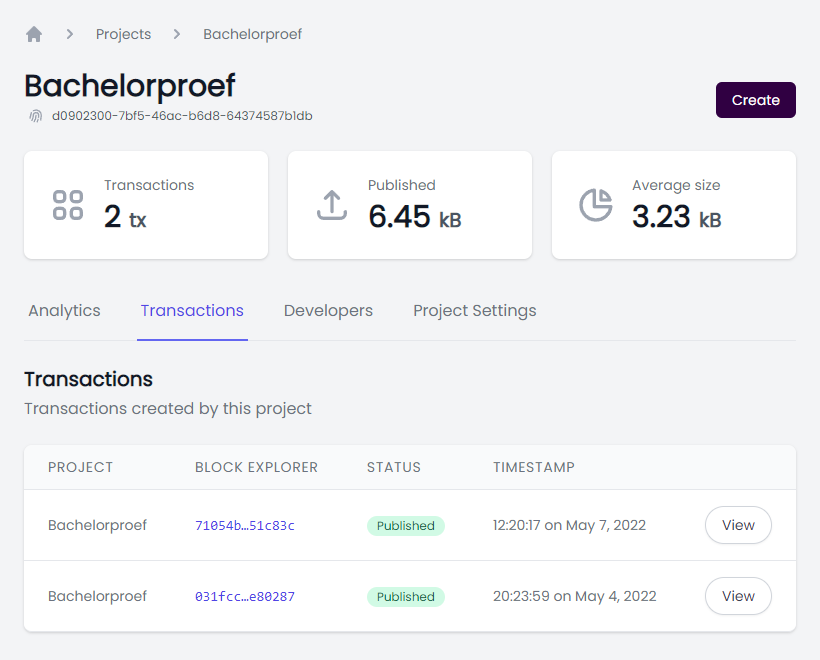
\includegraphics[width=\linewidth]{img/proof-of-concept/mintblue-project.png}
	\caption{\label{fig:mintblue-project}Project met transacties op het mintBlue-platform}
\end{figure}

Daarnaast biedt het platform ook een tool genaamd de ``composer''. Het is een grafische interface die helpt bij het opstellen van de juiste JSON voor een transactie. De GUI helpt om data, bestanden of scripts in te voeren. De bijhorende JSON wordt weergegeven.


\section{Kosten}
\label{sub:kosten}

Blockchains bieden op het vlak van opslagkosten een heel bijzondere manier om data te bewaren. Zoals werd opgemerkt in Subsectie \ref{sub:data-wegschrijven} -- \nameref{sub:data-wegschrijven} gaat het opslaan van data steeds gepaard met een transactie waarvoor een zekere fee betaald moet worden. Die fee moet miners ``aanmoedigen'' om de gepubliceerde transactie op te nemen in het volgende datablok. Eens een transactie deel uitmaakt van de blockchain, wordt het voor altijd bewaard door het collectieve netwerk. Opslaan in de blockchain gaat dus gepaard met een eenmalige kost van het publiceren, niet van het onderhoud\footnote{De kost van de infrastructuur waaruit het blockchain-netwerk is opgebouwd, wordt gedragen door de deelnemers die nodes voorzien. Deze hebben hun eigen incentive voor het draaiend houden van deze hardware, zoals het verdienen van fee's, aanbieden van een \textit{block explorers}, \textit{minen} van cryptomunten, ...}. 

Dit staat in contrast met andere -eerder klassieke- vormen van dataopslag. Opties zoals een eigen databank of cloud, gaan altijd gepaard met een zekere maintenance-kost die moet betaald worden door de partij die de data wilt stockeren. 
Vaak betekent dit een periodieke betalingen zoals een maandelijkse abonnementskost.

\subsection{mintBlue}
\label{sub:mintblue}

Dankzij bovenstaand gegeven rekent mintBlue af in functie van de hoeveelheid gepubliceerde data. Om iets op de blockchain te plaatsen, betaalt men eenmalig een vaste prijs per kilobyte. Die eenheidsprijs is afhankelijk van de afgesloten formule, met als bedoeling een zekere winstmarge te hebben op de benodigde fee's. Grotere transacties vereisen namelijk grotere fee's. Gelukkig (maar niet per toeval) maakt mintBlue gebruik van de BSV-blockchain, die een grote block size heeft van doorgaans 4GB\footnote{Er bestaat geen opgelegde limiet op de grootte van blokken. Op dit moment werken miners echter voornamelijk aan blokken van 4 GB.}. Daardoor zijn de fee's relatief klein. Voor de mock-factuur uit Subsectie \ref{sub:data-wegschrijven} -- \nameref{sub:data-wegschrijven} (van ongeveer 6000 B) bedroeg de fee 0.00000303 BSV, wat op het moment van schrijven ongeveer \euro 0.0002 waard is. De prijs die mintBlue doorrekent aan de klant hangt af van de afgesloten formule. Tabel~\ref{tab:mintblue-pricing} geeft de huidige specificaties weer. Opmerkelijk is dat er met \textit{basic} en \textit{enterprise} toch een bijkomende abonnementskost is. Deze opties brengen wel meer support met zich mee.

\begin{table}[H]
	\centering
	\begin{tabular}{@{}lccc@{}}
		\cmidrule(l){2-4}
		& \textbf{Free}                                                & \textbf{Basic} & \textbf{Enterprise} \\ \midrule
		Fee          & \euro 0                                                          & \euro 49 per month & custom              \\ \midrule
		Price per kB & \begin{tabular}[c]{@{}c@{}}\euro 0,02\\ (1 MB free)\end{tabular} & \euro 0,01         & \euro 0,005             \\ \midrule
		Projects     & 3                                                            & 10             & unlimited           \\ \midrule
		Support & community     & e-mail         & support manager     \\ \bottomrule
	\end{tabular}
	\caption{\label{tab:mintblue-pricing}Prijzen van mintBlue}
\end{table}

Met bovenstaande tabel kan een eerste schatting gemaakt worden van de kosten die 14IT zou moeten betalen om facturen op te slaan. Om een representatief beeld te schetsen, kan uitgegaan worden van een klant die maandelijks gemiddeld 350 facturen opmaakt. Na een steekproef werd de grootte van een doorsnee UBL-factuur ingeschat op 6 kB. Zelfs met een ruime marge is het veilig om de grootte van een gemiddelde transactie af te ronden op 8 kB. Bij een dergelijke klant lijkt de ``Free''-formule de beste optie. De 2800 kB aan data die maandelijks verwerkt moet worden, zou telkens ongeveer \euro 56 kosten. De ``Basic''-formule wordt voordeliger vanaf een omvang van 4900 kB, of ongeveer 613 facturen.

\subsection{Overwegingen}
\label{sub:overwegingen}

Bovenstaande inschatting maakt duidelijk dat de services van mintBlue op het eerste zicht duurder zijn de een traditionele cloud. Daarom moet ingeschat worden of de voordelen van NFT invoicing ook opwegen tegen de kosten. Hierbij kan men volgende overwegingen maken:

\begin{itemize}
	\item NFT invoicing kan aangeboden worden als bijkomende module van CPSolution en ook op die manier doorgerekend worden. Zo kan elke kmo voor zichzelf de inschatting maken of de voordelen wel opwegen tegenover de kosten. Indien voldoende klanten gebruik maken van deze module is een aangepaste ``Enterprise''-formule met mintBlue misschien wel aan de orde. Dat kan globaal genomen de kosten nog meer drukken.
	\item Eens data zich op de blockchain bevindt, blijft deze daar kosteloos en definitief aanwezig. Dat kan interessant zijn voor facturen aangezien deze volgens de wet minstens zeven jaar bijgehouden moeten worden. Bij cloud-oplossingen zou dit ook zeven jaar aan maintenance-kosten beteken. 
	\item Gezien de eenheidsprijs is een maand met weinig of geen facturen ook een maand met weinig of geen kosten. 
	\item NFT-invoicing biedt een alternatief voor de huidige EDI van CPSolution. Deze steunt op de services van Basware, wat ook gepaard gaat met een eigen kostenplaatje. In die context zijn de uitgaven aan mintblue niet bijkomend, maar vervangend.
\end{itemize}

Daarnaast is het niet meteen duidelijk welke invloed de koers van de BSV heeft op de kostprijs van mintBlue-transacties. CIO Pieter Den Dooven beweert althans dat het mogelijk is om een fixed price te blijven aanrekenen. Hiervoor werden contracten met datacenters gesloten. Daarnaast is BSV ook een blockchain dat een onbeperkt aantal transacties in eenzelfde blok toelaat, waardoor transaction fee's niet oplopen zoals bij BTC bijvoorbeeld het geval is.


\section{Kritische noot}
\label{sec:kritische-noot}

NFT invoicing heeft als opzet om een zekere vorm van onvervalsbaarheid te verkrijgen. Dat is dan ook gelukt: een onwijzigbare versie van de factuur staat definitief op de blockchain zoals de crediteur ze oorspronkelijk opmaakte. Fraudeurs kunnen echter nog op een andere manier proberen toeslaan: door de papieren factuur te onderscheppen en de QR-code te vervangen door een nieuwe QR-code die verwijst naar een eigen spookfactuur. De ontvanger zou de factuur goedkeuren op basis van de papieren versie, maar in het boekhoudsysteem zou de frauduleuze data binnensijpelen. Op die manier kan een overschrijving plaatsvinden naar de oplichter.

Een fraudeur zou hiermee echter een volledig spoor achterlaten van zijn bedrog. Een blockchain blijft in se nog steeds een keten van transacties. Bij elke transactie horen adressen die op hun beurt bij een zekere identity horen. Door het spoor aan transacties te volgen, zouden overheidsdiensten de oplichter kunnen vatten\footnote{Op die manier werden al criminelen opgespoord die de blockchain gebruikten als medium voor illegale praktijken zoals drugshandel en kindermisbruik.}. Hoewel het dus technisch mogelijk is om op deze manier spookfacturen uit te zenden, lijkt het er niet meteen op dat de blockchain hiervoor het geschikte medium is (vanuit de ogen van de fraudeur).

Bij mintBlue wordt in elk geval nog aan een oplossing met behulp van \textit{digital signatures} gewerkt. Hiervoor wordt een samenwerking op poten gezet met de Kamer van Koophandel. De KVK dataservice bevat alle actuele informatie uit het handelsregister. Door de publieke sleutel van elke onderneming op te nemen in de databank van de Kamer van Koophandel, wordt het voor iedereen mogelijk om te verifiëren dat de digitale factuur van de juiste partij afkomstig is. Met deze samenwerking berust men echter opnieuw op een zeker vorm van authoritaire derde partij. 







%%=============================================================================
%% Conclusie
%%=============================================================================

\chapter{Conclusie}
\label{ch:conclusie}

% TODO: Trek een duidelijke conclusie, in de vorm van een antwoord op de
% onderzoeksvra(a)g(en). Wat was jouw bijdrage aan het onderzoeksdomein en
% hoe biedt dit meerwaarde aan het vakgebied/doelgroep? 
% Reflecteer kritisch over het resultaat. In Engelse teksten wordt deze sectie
% ``Discussion'' genoemd. Had je deze uitkomst verwacht? Zijn er zaken die nog
% niet duidelijk zijn?
% Heeft het onderzoek geleid tot nieuwe vragen die uitnodigen tot verder 
%onderzoek?


Met dit onderzoek werd een antwoord gezocht op de vraag:

\begin{center}
	\textit{\textbf{``Hoe kunnen softwareontwikkelaars overgaan tot integratie van blockchaintechnologie voor de dataopslag van hun ERP-systeem?''}}
\end{center}

Dit werkstuk vormt op zich al een eerste deel van het antwoord op die vraag. Een softwareontwikkelaar die wil \textbf{overgaan tot} integratie, moet namelijk eerst
\begin{enumerate}
	\item een gefundeerd inzicht krijgen in de innerlijke werking van blockchains;
	\item het eigen ERP-systeem grondig in kaart brengen, om zo een zicht te krijgen op wat voor verbetering vatbaar is;
	\item de vorige twee items aaneenknopen door naar die blockchain-toepassingen te zoeken die potientieel vertonen binnen ERP.
\end{enumerate}

Deze bachelorproef vervult alvast deze drie voorwaarden voor 14IT. De hoofdstukken drie tot en met vijf werden zodanig opgesteld dat de lezer er vlot de nodige bagage mee kan vergaren. Dat geldt vooral binnen 14IT, maar ook voor softwareontwikkelaars in het algemeen.

De onderzoeksvraag onstond echter vanuit de concrete casus van CPSolution. Als gevolg moet er ook een concreet besluit getrokken worden. Bovenvermelde hoofdstukken helpen de lezer wel bij het overgaan tot integratie, maar nog niet bij het \textbf{integreren} zelf. Dat gebeurt in het zesde hoofdstuk.

De meest rudimentaire conclusie is dat het effectief mogelijk is om als kmo de data van een eigen ERP-systeem op te slaan in een blockchain. Dit vormde bij aanvang van het onderzoek nog een groot vraagteken, maar werd met de \textit{proof of concept} positief bevestigd. Een blockchain zoals BSV staat open voor allerhande data. Onder de vorm van een \textit{data-carrying} output kon data, zoals die uit het ERP-systeem, op de blockchain geplaatst worden. 

De suggestie van dit onderzoek is om bovenstaand principe in te schakelen voor het stockeren van digitale facturen. De data die dan op de blockchain komt is een geëncrypteerd UBL-bestand van die factuur. CPSolution beschikt al over de functionaliteiten om een factuur onder dat formaat te exporteren. Als bestuurslid van UBL.BE, kan 14IT zo de missie van de werkgroep misschien zelfs nog meer kracht bijzetten.

Dit gegeven biedt tevens een nuttige \textit{use case}, genaamd NFT invoicing. Een API die data van de keten leest en daarna decrypteert, biedt de debiteur een endpoint om de factuur gemakkelijk op te halen. Op die manier kunnen e-invoices uitgewisseld worden via de openbare ``databank'' die men de blockchain noemt. Het biedt een alternatief voor de huidige manier waarop CPSolution aan EDI doet. Dankzij de \textit{incorruptibility} en \textit{transparancy} vormt de blockchain een ``single source of truth'' voor onderhandelende partijen.

De API-call biedt als voordeel dat het als QR-code op papier kan gezet worden. Zo komt deze oplossing ook tegemoet aan de wens van bedrijven die facturen op papier valideren. Met een eenvoudige scan krijgt de ontvanger meteen de ongewijzigde, digitale tweeling van het document. Mits een check op identity toe te voegen, kan de ontvanger ook valideren dat deze van de correcte partij komt.

Een API zoals hierboven beschreven wordt aangeboden door het bedrijf mintBlue. Deze omvat ook methodes voor het wegschrijven van data in de blockchain. Met een dergelijke service zou 14IT NFT invoicing als module van CPSolution kunnen integreren, zonder zelf extra infrastructuur op te stellen of te onderhouden. Daarvoor moet enkel de business logica geprogrammeerd worden rond de aangeboden API-calls ``naar de blockchain''. Dat kan in C\# en zou het vervolg van dit onderzoek kunnen vormen.

%%=============================================================================
%% Bijlagen
%%=============================================================================

\appendix
\renewcommand{\chaptername}{Appendix}

%%---------- Onderzoeksvoorstel -----------------------------------------------

\chapter{Onderzoeksvoorstel}
\label{ch:onderzoeksvoorstel}

Het onderwerp van deze bachelorproef is gebaseerd op een onderzoeksvoorstel dat vooraf werd beoordeeld door de promotor. Dat voorstel is opgenomen in deze bijlage.

% Verwijzing naar het bestand met de inhoud van het onderzoeksvoorstel
%---------- Inleiding ---------------------------------------------------------

\section{Introductie} % The \section*{} command stops section numbering
\label{sec:introductie}

In 1982 introduceerde cryptograaf David Chaum een protocol dat de grondslag vormde van wat men vandaag een blockchain noemt. De eerste werkzame implementatie werd pas een feit toen Satoshi Nakamoto in 2008 de eerste gedecentraliseerde digitale munt \textit{Bitcoin} in het leven riep. Sindsdien wordt de term ``blockchain'' alom gebruikt als buzzwoord voor alles wat met \textit{cryptocurrencies} te maken heeft. Zo ziet men echter enkel het topje van de ijsberg. Ook in andere branches ziet men namelijk steeds meer opportuniteiten voor deze nieuwe vorm van dataopslag. De verwachting is dat blockchain nog meer te bieden heeft dan wat op dit moment al gekend is. Daarom zoekt men vanuit allerlei frisse invalshoeken naar vernieuwende toepassingen voor deze technologie. Ondernemers stellen zich de vraag of blockchain ook voor hun een meerwaarde in petto heeft. Dit is ook het geval bij softwareontwikkelaar 14IT. In het verdere voorstel en onderzoek zal aan bod komen wat deze ``meerwaarde'' juist inhoudt.

14IT ontwikkelde het ERP-syteem ``CPSolution'' voor zijn klanten (kmo's). Een deel van het takenpakket bestaat uit het verder ontwikkelen en onderhouden van deze software. In dit kader van continuous improvement ontstond de interesse in dit onderwerp. De vraag stelt zich of het programma verbeterd of uitgebreid kan worden door in te zetten op blockchain.

Aangezien het onderwerp van hieruit werd aangereikt, zal deze bedrijfscasus ook de rode draad vormen die door het werkstuk loopt. Hoewel het thema \textit{blockchain for ERP} in eerste instantie vanop \textit{high-level} benaderd zal worden, is het de bedoeling om doorheen het proces steeds concreter te gaan. Zo hoort uiteindelijk een resultaat behaald te worden dat praktisch inzetbaar is, in het bijzonder door 14IT.


De doelstelling, zoals hierboven beschreven, kan herleid worden naar volgende onderzoeksvraag:

\begin{center}
	\textit{\textbf{``Hoe kunnen softwareontwikkelaars overgaan tot integratie van blockchaintechnologie voor de dataopslag van een ERP-systeem?''}}
\end{center}

In sectie \ref{sec:methodologie} - \nameref{sec:methodologie} staat beschreven hoe ik deze onderzoeksvraag op een systematische manier zal trachten te beantwoorden.




%---------- Stand van zaken ---------------------------------------------------
\section{Literatuurstudie}
\label{sec:state-of-the-art}

\subsection{Wat is blockchain?}
\label{sub:wat-is-blockchain}

Een blockchain kan voorgesteld worden als een keten van datablokken, waarin nieuwe data enkel kan toegevoegd worden onder de vorm van een nieuw blok aan het einde van de keten. Het is een techniek om transacties zodanig bij te houden dat deze later niet meer vervalst kunnen worden. Deze eigenschap, genaamd \textit{immutability}, wordt mogelijk gemaakt door het gedecentraliseerde karakter van de blokketen. Het is namelijk zo dat de data wordt opgeslagen in een speciale, gedistribueerde database die men een \textit{distributed ledger} noemt. Hierin worden de transacties verspreid over verschillende toestellen (\textit{nodes}) waarvoor geen centrale autoriteit bestaat. Participanten hoeven de betrouwbaarheid van tussenpersonen of andere deelnemers niet meer te beoordelen, aangezien de betrouwbaarheid van het systeem als geheel al volstaat~\autocite{Nofer2017}. Die betrouwbaarheid wordt verwezenlijkt door de slimme implementatie van blockchain die gebruik maakt van cryptografie, iets wat aan bod zal komen in een uitgebreidere literatuurstudie (zie sectie \ref{sec:methodologie} - \nameref{sec:methodologie}).



\subsection{Perspectieven}
\label{sub:perspectieven}

In de oorspronkelijke toepassing stond een transactie voor de bitcoin-overdracht van een partij naar een andere~\autocite{Pierro2017}. 

Er zijn echter veel meer transacties denkbaar dan eenvoudige gelduitwisselingen. Andere voorbeelden zijn het ondertekenen van slimme contracten, uitwisselen van aandelen, obligaties of hypotheken enzovoort (Blockchain 2.0). Blockchain 3.0 zoekt zelfs naar toepassingen binnen de overheid, wetenschap en kunst~\autocite{Swan2015}.

University of Cambridge gebruikte data van meer dan 200 start-ups, financiële ondernemingen, banken en andere publieke instituties om na te gaan welke toepassingen al bestaan voor \textit{distributed ledger} technologie. Men kwam tot een lijst van 132 use cases, gegroepeerd per sector. Hoewel men een grote aanwezigheid vaststelde van banken en betalingen, stelde men een toenemende interesse vast voor toepassingen zoals de \textit{supply chain}~\autocite{Hileman2017}.

Rejeb ziet een kans om ERP-systemen van verschillende ontwikkelaars en stakeholders samen te brengen op eenzelfde platform. Blockchain zou een dergelijk ERP-netwerk mogelijk kunnen maken~\autocite{Rejeb2018}.

Zoals eerder vermeld is een blockchain \textit{immutable} en gedecentraliseerd. Use cases voor het ERP-systeem van een kmo zullen een meerwaarde bieden, wanneer deze twee eigenschappen benut worden. Zo kan men bijvoorbeeld transacties omtrent facturen opnemen in een \textit{distributed ledger}. Een klant die dan een digitale factuur ontvangt, kan dankzij de \textit{immutability} nagaan of deze effectief van de afzender komt en dus geen \textit{spoofing} is.


\subsection{State-of-the-art}
\label{sub:state-of-the-art}

De huidige platformen voor blockchain staan nog in hun kinderschoenen. Nog zo recent als 2016 waren blockchain technologieën, die voor de markt bestemd waren, in een experimentele fase~\autocite{Davidson2016}.

Ondertussen zijn er al spelers die blockchainplatformen aanbieden op de markt (zoals mintBlue). Deze ondernemingen worstelden lang met uitdagingen rond privacy en schaalbaarheid, waarvoor mogelijke oplossingen bedacht werden~\autocite{Kaptijn}. Er zijn al enkele voorbeelden van ondernemingen die mee op de kar springen, zoals aanbieder van online boekhoudsoftware Yuki. Ook binnen de Vlaamse overheid zijn projecten lopend voor verschillende blockchain-toepassingen~\autocite{Schiltz2018}.


% Voor literatuurverwijzingen zijn er twee belangrijke commando's:
% \autocite{KEY} => (Auteur, jaartal) Gebruik dit als de naam van de auteur
%   geen onderdeel is van de zin.
% \textcite{KEY} => Auteur (jaartal)  Gebruik dit als de auteursnaam wel een
%   functie heeft in de zin (bv. ``Uit onderzoek door Doll & Hill (1954) bleek
%   ...'')


%---------- Methodologie ------------------------------------------------------
\section{Methodologie}
\label{sec:methodologie}

De onderzoeksvraag (zoals beschreven in sectie \ref{sec:introductie} - \nameref{sec:introductie}) geeft de essentie van het onderzoek weer. Het systematisch beantwoorden van onderstaande \textbf{deelvragen} zou mij in staat moeten stellen om de bijhorende doelstelling te behalen.

\begin{enumerate}
	\item Wat is een blockchain?
	\item Hoe wordt de data van een ERP-syteem opgeslagen? (\textit{as is})
	\item Welke mogelijkheden biedt blockchain voor een ERP-systeem?
	\item Hoe kunnen softwareontwikkelaars de data van het ERP-systeem opslaan in een blockchain? (\textit{to be})
	
\end{enumerate}

Zoals hiervoor beschreven is het de bedoeling om, vertrekkende vanuit een \textit{high level}, zo snel mogelijk concreet toe te werken naar de bedrijfscasus. Die benadering weerspiegelt zich in de opgesomde deelvragen en de volgorde ervan.

Een \textbf{literatuurstudie} vormt de basis van elk van deze deelvragen en is daarom de eerste fase van het onderzoek. Hierin kan uitgespit worden
\begin{enumerate}
	\item hoe de werking en implementatie van een blockchain eruit ziet; welke soorten blockchains bestaan;
	\item welke eisen en aandachtspunten er zijn qua dataopslag in een ERP-context; welke noden en kansen er nog bestaan bij het opslaan van data omtrent de \textit{supply chain}; use cases van blockchains in andere bedrijven;
	\item welke voor- en nadelen een blockchain met zich meebrengt; 
	\item welke manieren er bestaan om data vast te leggen in een blockchain; welke kosten er gepaard gaan bij deze integratie.
\end{enumerate}

Het spreekt voor zich dat louter een literatuurstudie niet volstaat om alle deelvragen naar behoren te behandelen. 
De tweede deelvraag biedt zich aan als gelegenheid om de \textit{as is} situatie in kaart te brengen. Een \textbf{\textit{case study}} van \textit{CPSolution} is hier wel op zijn plaats. Ook dient onderzocht te worden welke mogelijkheden al gebruikt worden op de markt en voor welke use cases. Dit kan aan de hand van een soort kleinschalige \textbf{marktanalyse}, horend bij de derde deelvraag. Op dat moment zou het mogelijk moeten zijn om de inschatting te maken of blockchain een meerwaarde kan bieden. In de laatste deelvraag proberen we de \textit{to-be} situatie in kaart te brengen.


%---------- Verwachte resultaten ----------------------------------------------
\section{Verwachte resultaten}
\label{sec:verwachte_resultaten}

Zoals al eerder vermeld, moet het onderzoek resulteren in iets wat praktisch bruikbaar is binnen de softwareontwikkeling. Hier ligt dan ook de focus van de bachelorproef.

Enerzijds zal het resulterend \textbf{werkstuk} de lezer in staat stellen om zich vlot in te werken in het onderwerp. Aan de hand van de werking, \textit{pros and cons}, opportuniteiten en platformen van \textit{blockchain for ERP} die hierin beschreven zullen worden, kan men beslissen of men wil overgaan tot integratie. Er valt voorlopig al veel te vinden over blockchain, waarvan niet alles even interessant is in de context van een ERP-systeem. Het eindresultaat moet 14IT helpen om door de bomen het bos te zien.

Anderzijds moet er ook iets voorzien worden voor die softwareontwikkelaars die de stap effectief wensen te zetten. Om een houvast te bieden tijdens die overgang zou een vooropgestelde \textbf{procedure} uitgewerkt kunnen worden. Beeld hierbij een soort plan (van aanpak) in dat de ondernemer helpt om stap per stap naar de \textit{to-be} situatie toe te werken. Het kostenplaatje van heel dit gegeven mag hierin niet ontbreken.


%---------- Verwachte conclusies ----------------------------------------------
\section{Verwachte conclusies}
\label{sec:verwachte_conclusies}

De \emph{state-of-the-art} rondom het gekozen onderzoeksdomein laat vermoeden dat blockchain veel in petto heeft voor allerhande toepassingen. Ook voor ERP-systemen klinkt het veelbelovend.	Vermoedelijk zullen toepassingen op het niveau van Blockchain 2.0 momenteel het meest aan de orde zijn voor kmo's zoals 14IT. Dit wordt dan het scope-gebied van het onderzoek.

Het is hoogstwaarschijnlijk uitvoerbaar om de data rond ERP vast te leggen in een blockchain. Het is niet ondenkbaar dat dit ook een meerwaarde zal hebben. De mate waarin dit ook opweegt tegen de bijhorende investeringen in tijd en kapitaal vormt voorlopig een groter vraagteken. Daarom is het moeilijk om nu al in te schatten of die omschakeling naar blockchain ook rendabel is (voor 14IT). De uitwerking van deze bachelorproef zal daar hopelijk bij helpen.



%%---------- Andere bijlagen --------------------------------------------------

\chapter{Modules van CPSolution}
\label{ch:modules-van-cpsolution}

\textbf{Basismodules}
Connecties (Klanten - Leveranciers)/Producten - Productgroepen - Samengestelde producten - Taksen(Recupel, bebat,..)
Management (OptionLists - Accounting - Taxen) - Licentiebeheer - Bedrijfsparameters - Rapportinstellingen - Basisinstellingen

\textbf{Logistiek}
Verkooporders-Magazijnbon-Leveringsnota-Factuur/Creditnota-Verzamelfactuur
Verkoopoffertes
Recurrente Verkoopregistratie (abonnementen-afroeporders)
Prijzen - kortingen - prijsafspraken Verkoop
Aankooporders - Voorraadregistratie(pallet-product) - Factuur/Creditnota
Aankoopoffertes
Recurrente Aankoopregistratie (abonnementen- afroeporders)
Prijzen - kortingen - prijsafspraken Inkoop
Verkoop/Aankoop scenario's (template)
Contactbeheer (personen - bedrijven - afdelingen)
Lotnummers(vervaldatum)/serienummers
Transport (paletten - vervoersdocumenten)
Klantenkaart/Service kaart
Consignatie stock/verkoop
Verhuur
Verkoop/Inkoop orders koppeling
Koppeling met NordicID scanner
Eenheden/Unit Productmatrix-conversie tabel
Productmatrix X-Y as (bijv. maten/Aleuren)
Formule/Calculatie
EID Koppeling
Analytisch Boekhouden

\textbf{Financieel}
Betalingsregistratie
Kassa
Kassa Koppeling betaalterminal

\textbf{Productie}
Productieplanning
Ingaveschermen productie
Productieoverzicht-koppeling verkooporder
Aansturing productielabels

\textbf{Stockbeheer}
Stocktransactie - Magazijnen - Locaties - stockproductie

\textbf{Connectiviteitsmodules}
Vertaalmodule
Tekstimport (CPSolution/Venice/Multivers)
Venice (import/export)
Multivers (import/export)
Certipost (import/export)
Webshop/Website connection
Webshop
Website CMS
Excel Import
ExpertM (export)
Server Client connectie


\chapter{Mock-factuur}
\label{ch:mock-factuur}

\begin{figure}[]
	\includegraphics[width=\linewidth]{img/bijlagen/mock-factuur.pdf}
\end{figure}

%%---------- Referentielijst --------------------------------------------------

\printbibliography[heading=bibintoc]

\end{document}
